%&preformat-disser
\RequirePackage[l2tabu,orthodox]{nag} % Раскомментировав, можно в логе получать рекомендации относительно правильного использования пакетов и предупреждения об устаревших и нерекомендуемых пакетах
% Формат А4, 14pt (ГОСТ Р 7.0.11-2011, 5.3.6)
\documentclass[a4paper,14pt,oneside,openany]{memoir}

\input{common/setup}            % общие настройки шаблона
\input{common/packages}         % Пакеты общие для диссертации и автореферата
\synopsisfalse                      % Этот документ --- не автореферат
\input{Dissertation/dispackages}    % Пакеты для диссертации
\input{Dissertation/userpackages}   % Пакеты для специфических пользовательских задач

\input{Dissertation/setup}      % Упрощённые настройки шаблона

\input{common/newnames}         % Новые переменные, для всего проекта

%%% Основные сведения %%%
\newcommand{\thesisAuthorLastName}{Владимиров}
\newcommand{\thesisAuthorOtherNames}{Константин Игоревич}
\newcommand{\thesisAuthorInitials}{К.\,И.}
\newcommand{\thesisAuthor}             % Диссертация, ФИО автора
{%
    \texorpdfstring{% \texorpdfstring takes two arguments and uses the first for (La)TeX and the second for pdf
        \thesisAuthorLastName~\thesisAuthorOtherNames% так будет отображаться на титульном листе или в тексте, где будет использоваться переменная
    }{%
        \thesisAuthorLastName, \thesisAuthorOtherNames% эта запись для свойств pdf-файла. В таком виде, если pdf будет обработан программами для сбора библиографических сведений, будет правильно представлена фамилия.
    }
}
\newcommand{\thesisAuthorShort}        % Диссертация, ФИО автора инициалами
{\thesisAuthorInitials~\thesisAuthorLastName}
%\newcommand{\thesisUdk}                % Диссертация, УДК
%{004.4'422}
\newcommand{\thesisTitle}              % Диссертация, название
{Исследование и разработка методов оптимизации работы с памятью в компиляторах для гетерогенных вычислительных систем с векторной архитектурой}
\newcommand{\thesisSpecialtyNumber}    % Диссертация, специальность, номер
{2.3.5}
\newcommand{\thesisSpecialtyTitle}     % Диссертация, специальность, название (название взято с сайта ВАК для примера)
{Математическое и программное обеспечение вычислительных систем, комплексов и компьютерных сетей}
\newcommand{\thesisDegree}             % Диссертация, ученая степень
{кандидата технических наук}
\newcommand{\thesisDegreeShort}        % Диссертация, ученая степень, краткая запись
{канд. техн. наук}
\newcommand{\thesisCity}               % Диссертация, город написания диссертации
{Москва}
\newcommand{\thesisYear}               % Диссертация, год написания диссертации
{\the\year}
\newcommand{\thesisOrganization}       % Диссертация, организация
{Федеральное государственное автономное образовательное учреждение высшего
образования <<Московский физико-технический институт (национальный исследовательский университет)>> (МФТИ, Физтех)}
\newcommand{\thesisOrganizationShort}  % Диссертация, краткое название организации для доклада
{\fixme{МФТИ}}

\newcommand{\thesisInOrganization}     % Диссертация, организация в предложном падеже: Работа выполнена в ...
{ПАО ИНЭУМ им. И.С. Брука}

%% \newcommand{\supervisorDead}{}           % Рисовать рамку вокруг фамилии
\newcommand{\supervisorFio}              % Научный руководитель, ФИО
{Плоткин Арнольд Леонидович}
\newcommand{\supervisorRegalia}          % Научный руководитель, регалии
{доктор технических наук, профессор}
\newcommand{\supervisorFioShort}         % Научный руководитель, ФИО
{А.\,Л.~Плоткин}
\newcommand{\supervisorRegaliaShort}     % Научный руководитель, регалии
{д.~т.~н.,~проф.}

%% \newcommand{\supervisorTwoDead}{}        % Рисовать рамку вокруг фамилии
%% \newcommand{\supervisorTwoFio}           % Второй научный руководитель, ФИО
%% {\fixme{Фамилия Имя Отчество}}
%% \newcommand{\supervisorTwoRegalia}       % Второй научный руководитель, регалии
%% {\fixme{уч. степень, уч. звание}}
%% \newcommand{\supervisorTwoFioShort}      % Второй научный руководитель, ФИО
%% {\fixme{И.\,О.~Фамилия}}
%% \newcommand{\supervisorTwoRegaliaShort}  % Второй научный руководитель, регалии
%% {\fixme{уч.~ст.,~уч.~зв.}}

\newcommand{\opponentOneFio}           % Оппонент 1, ФИО
{\fixme{Фамилия Имя Отчество}}
\newcommand{\opponentOneRegalia}       % Оппонент 1, регалии
{\fixme{доктор физико-математических наук, профессор}}
\newcommand{\opponentOneJobPlace}      % Оппонент 1, место работы
{\fixme{Не очень длинное название для места работы}}
\newcommand{\opponentOneJobPost}       % Оппонент 1, должность
{\fixme{старший научный сотрудник}}

\newcommand{\opponentTwoFio}           % Оппонент 2, ФИО
{\fixme{Фамилия Имя Отчество}}
\newcommand{\opponentTwoRegalia}       % Оппонент 2, регалии
{\fixme{кандидат физико-математических наук}}
\newcommand{\opponentTwoJobPlace}      % Оппонент 2, место работы
{\fixme{Основное место работы c длинным длинным длинным длинным названием}}
\newcommand{\opponentTwoJobPost}       % Оппонент 2, должность
{\fixme{старший научный сотрудник}}

%% \newcommand{\opponentThreeFio}         % Оппонент 3, ФИО
%% {\fixme{Фамилия Имя Отчество}}
%% \newcommand{\opponentThreeRegalia}     % Оппонент 3, регалии
%% {\fixme{кандидат физико-математических наук}}
%% \newcommand{\opponentThreeJobPlace}    % Оппонент 3, место работы
%% {\fixme{Основное место работы c длинным длинным длинным длинным названием}}
%% \newcommand{\opponentThreeJobPost}     % Оппонент 3, должность
%% {\fixme{старший научный сотрудник}}

\newcommand{\leadingOrganizationTitle} % Ведущая организация, дополнительные строки. Удалить, чтобы не отображать в автореферате
{\fixme{Федеральное государственное бюджетное образовательное учреждение высшего
профессионального образования с~длинным длинным длинным длинным названием}}

\newcommand{\defenseDate}              % Защита, дата
{\fixme{DD mmmmmmmm YYYY~г.~в~XX часов}}
\newcommand{\defenseCouncilNumber}     % Защита, номер диссертационного совета
{\fixme{Д\,123.456.78}}
\newcommand{\defenseCouncilTitle}      % Защита, учреждение диссертационного совета
{\fixme{Название учреждения}}
\newcommand{\defenseCouncilAddress}    % Защита, адрес учреждение диссертационного совета
{\fixme{Адрес}}
\newcommand{\defenseCouncilPhone}      % Телефон для справок
{\fixme{+7~(0000)~00-00-00}}

\newcommand{\defenseSecretaryFio}      % Секретарь диссертационного совета, ФИО
{\fixme{Фамилия Имя Отчество}}
\newcommand{\defenseSecretaryRegalia}  % Секретарь диссертационного совета, регалии
{\fixme{д-р~физ.-мат. наук}}            % Для сокращений есть ГОСТы, например: ГОСТ Р 7.0.12-2011 + http://base.garant.ru/179724/#block_30000

\newcommand{\synopsisLibrary}          % Автореферат, название библиотеки
{\fixme{Название библиотеки}}
\newcommand{\synopsisDate}             % Автореферат, дата рассылки
{\fixme{DD mmmmmmmm}\the\year~года}

% To avoid conflict with beamer class use \providecommand
\providecommand{\keywords}%            % Ключевые слова для метаданных PDF диссертации и автореферата
{}
             % Основные сведения
\input{common/fonts}            % Определение шрифтов (частичное)
\input{common/styles}           % Стили общие для диссертации и автореферата
\input{Dissertation/disstyles}  % Стили для диссертации
\input{Dissertation/userstyles} % Стили для специфических пользовательских задач

%%% Библиография. Выбор движка для реализации %%%
% Здесь только проверка установленного ключа. Сама настройка выбора движка
% размещена в common/setup.tex
\ifnumequal{\value{bibliosel}}{0}{%
    \input{biblio/predefined}   % Встроенная реализация с загрузкой файла через движок bibtex8
}{
    %%% Реализация библиографии пакетами biblatex и biblatex-gost с использованием движка biber %%%

\usepackage{csquotes} % biblatex рекомендует его подключать. Пакет для оформления сложных блоков цитирования.
%%% Загрузка пакета с основными настройками %%%
\makeatletter
\ifnumequal{\value{draft}}{0}{% Чистовик
\usepackage[%
backend=biber,% движок
bibencoding=utf8,% кодировка bib файла
sorting=none,% настройка сортировки списка литературы
style=gost-numeric,% стиль цитирования и библиографии (по ГОСТ)
language=autobib,% получение языка из babel/polyglossia, default: autobib % если ставить autocite или auto, то цитаты в тексте с указанием страницы, получат указание страницы на языке оригинала
autolang=other,% многоязычная библиография
clearlang=true,% внутренний сброс поля language, если он совпадает с языком из babel/polyglossia
defernumbers=true,% нумерация проставляется после двух компиляций, зато позволяет выцеплять библиографию по ключевым словам и нумеровать не из большего списка
sortcites=true,% сортировать номера затекстовых ссылок при цитировании (если в квадратных скобках несколько ссылок, то отображаться будут отсортированно, а не абы как)
doi=false,% Показывать или нет ссылки на DOI
isbn=false,% Показывать или нет ISBN, ISSN, ISRN
]{biblatex}[2016/09/17]
\ltx@iffilelater{biblatex-gost.def}{2017/05/03}%
{\toggletrue{bbx:gostbibliography}%
\renewcommand*{\revsdnamepunct}{\addcomma}}{}
}{%Черновик
\usepackage[%
backend=biber,% движок
bibencoding=utf8,% кодировка bib файла
sorting=none,% настройка сортировки списка литературы
% defernumbers=true, % откомментируйте, если требуется правильная нумерация ссылок на литературу в режиме черновика. Замедляет сборку
]{biblatex}[2016/09/17]%
}
\makeatother

\providebool{blxmc} % biblatex version needs and has MakeCapital workaround
\boolfalse{blxmc} % setting our new boolean flag to default false
\ifxetexorluatex
\else
% Исправление случая неподдержки знака номера в pdflatex
    \DefineBibliographyStrings{russian}{number={\textnumero}}

% Исправление случая отсутствия прописных букв в некоторых случаях
% https://github.com/plk/biblatex/issues/960#issuecomment-596658282
    \ifdefmacro{\ExplSyntaxOn}{}{\usepackage{expl3}}
    \makeatletter
    \ltx@ifpackagelater{biblatex}{2020/02/23}{
    % Assuming this version of biblatex defines MakeCapital correctly
    }{
        \ltx@ifpackagelater{biblatex}{2019/12/01}{
            % Assuming this version of biblatex defines MakeCapital incorrectly
            \usepackage{expl3}[2020/02/25]
            \@ifpackagelater{expl3}{2020/02/25}{
                \booltrue{blxmc} % setting our new boolean flag to true
            }{}
        }{}
    }
    \makeatother
    \ifblxmc
        \typeout{Assuming this version of biblatex defines MakeCapital
        incorrectly}
        \usepackage{xparse}
        \makeatletter
        \ExplSyntaxOn
        \NewDocumentCommand \blx@maketext@lowercase {m}
          {
            \text_lowercase:n {#1}
          }

        \NewDocumentCommand \blx@maketext@uppercase {m}
          {
            \text_uppercase:n {#1}
          }

        \RenewDocumentCommand \MakeCapital {m}
          {
            \text_titlecase_first:n {#1}
          }
        \ExplSyntaxOff

        \protected\def\blx@biblcstring#1#2#3{%
          \blx@begunit
          \blx@hyphenreset
          \blx@bibstringsimple
          \lowercase{\edef\blx@tempa{#3}}%
          \ifcsundef{#2@\blx@tempa}
            {\blx@warn@nostring\blx@tempa
             \blx@endnounit}
            {#1{\blx@maketext@lowercase{\csuse{#2@\blx@tempa}}}%
             \blx@endunit}}

        \protected\def\blx@bibucstring#1#2#3{%
          \blx@begunit
          \blx@hyphenreset
          \blx@bibstringsimple
          \lowercase{\edef\blx@tempa{#3}}%
          \ifcsundef{#2@\blx@tempa}
            {\blx@warn@nostring\blx@tempa
             \blx@endnounit}
            {#1{\blx@maketext@uppercase{\csuse{#2@\blx@tempa}}}%
             \blx@endunit}}
        \makeatother
    \fi
\fi

\ifsynopsis
\ifnumgreater{\value{usefootcite}}{0}{
    \ExecuteBibliographyOptions{autocite=footnote}
    \newbibmacro*{cite:full}{%
        \printtext[bibhypertarget]{%
            \usedriver{%
                \DeclareNameAlias{sortname}{default}%
            }{%
                \thefield{entrytype}%
            }%
        }%
        \usebibmacro{shorthandintro}%
    }
    \DeclareCiteCommand{\smartcite}[\mkbibfootnote]{%
        \usebibmacro{prenote}%
    }{%
        \usebibmacro{citeindex}%
        \usebibmacro{cite:full}%
    }{%
        \multicitedelim%
    }{%
        \usebibmacro{postnote}%
    }
}{}
\fi

%%% Подключение файлов bib %%%
\addbibresource[label=bl-external]{biblio/vla-external.bib}
\addbibresource[label=bl-author]{biblio/vla-author.bib}

\iffalse
\addbibresource[label=bl-registered]{biblio/vla-registered.bib}
\fi

%http://tex.stackexchange.com/a/141831/79756
%There is a way to automatically map the language field to the langid field. The following lines in the preamble should be enough to do that.
%This command will copy the language field into the langid field and will then delete the contents of the language field. The language field will only be deleted if it was successfully copied into the langid field.
\DeclareSourcemap{ %модификация bib файла перед тем, как им займётся biblatex
    \maps{
        \map{% перекидываем значения полей language в поля langid, которыми пользуется biblatex
            \step[fieldsource=language, fieldset=langid, origfieldval, final]
            \step[fieldset=language, null]
        }
        \map{% перекидываем значения полей numpages в поля pagetotal, которыми пользуется biblatex
            \step[fieldsource=numpages, fieldset=pagetotal, origfieldval, final]
            \step[fieldset=numpages, null]
        }
        \map{% перекидываем значения полей pagestotal в поля pagetotal, которыми пользуется biblatex
            \step[fieldsource=pagestotal, fieldset=pagetotal, origfieldval, final]
            \step[fieldset=pagestotal, null]
        }
        \map[overwrite]{% перекидываем значения полей shortjournal, если они есть, в поля journal, которыми пользуется biblatex
            \step[fieldsource=shortjournal, final]
            \step[fieldset=journal, origfieldval]
            \step[fieldset=shortjournal, null]
        }
        \map[overwrite]{% перекидываем значения полей shortbooktitle, если они есть, в поля booktitle, которыми пользуется biblatex
            \step[fieldsource=shortbooktitle, final]
            \step[fieldset=booktitle, origfieldval]
            \step[fieldset=shortbooktitle, null]
        }
        \map{% если в поле medium написано "Электронный ресурс", то устанавливаем поле media, которым пользуется biblatex, в значение eresource.
            \step[fieldsource=medium,
            match=\regexp{Электронный\s+ресурс},
            final]
            \step[fieldset=media, fieldvalue=eresource]
            \step[fieldset=medium, null]
        }
        \map[overwrite]{% стираем значения всех полей issn
            \step[fieldset=issn, null]
        }
        \map[overwrite]{% стираем значения всех полей abstract, поскольку ими не пользуемся, а там бывают "неприятные" латеху символы
            \step[fieldsource=abstract]
            \step[fieldset=abstract,null]
        }
        \map[overwrite]{ % переделка формата записи даты
            \step[fieldsource=urldate,
            match=\regexp{([0-9]{2})\.([0-9]{2})\.([0-9]{4})},
            replace={$3-$2-$1$4}, % $4 вставлен исключительно ради нормальной работы программ подсветки синтаксиса, которые некорректно обрабатывают $ в таких конструкциях
            final]
        }
        \map[overwrite]{ % стираем ключевые слова
            \step[fieldsource=keywords]
            \step[fieldset=keywords,null]
        }
        % реализация foreach различается для biblatex v3.12 и v3.13.
        % Для версии v3.13 эта конструкция заменяет последующие 7 структур map
        % \map[overwrite,foreach={authorvak,authorscopus,authorwos,authorconf,authorother,authorparent,authorprogram}]{ % записываем информацию о типе публикации в ключевые слова
        %     \step[fieldsource=$MAPLOOP,final=true]
        %     \step[fieldset=keywords,fieldvalue={,biblio$MAPLOOP},append=true]
        % }
        \map[overwrite]{ % записываем информацию о типе публикации в ключевые слова
            \step[fieldsource=authorvak,final=true]
            \step[fieldset=keywords,fieldvalue={,biblioauthorvak},append=true]
        }
        \map[overwrite]{ % записываем информацию о типе публикации в ключевые слова
            \step[fieldsource=authorscopus,final=true]
            \step[fieldset=keywords,fieldvalue={,biblioauthorscopus},append=true]
        }
        \map[overwrite]{ % записываем информацию о типе публикации в ключевые слова
            \step[fieldsource=authorwos,final=true]
            \step[fieldset=keywords,fieldvalue={,biblioauthorwos},append=true]
        }
        \map[overwrite]{ % записываем информацию о типе публикации в ключевые слова
            \step[fieldsource=authorconf,final=true]
            \step[fieldset=keywords,fieldvalue={,biblioauthorconf},append=true]
        }
        \map[overwrite]{ % записываем информацию о типе публикации в ключевые слова
            \step[fieldsource=authorother,final=true]
            \step[fieldset=keywords,fieldvalue={,biblioauthorother},append=true]
        }
        \map[overwrite]{ % записываем информацию о типе публикации в ключевые слова
            \step[fieldsource=authorpatent,final=true]
            \step[fieldset=keywords,fieldvalue={,biblioauthorpatent},append=true]
        }
        \map[overwrite]{ % записываем информацию о типе публикации в ключевые слова
            \step[fieldsource=authorprogram,final=true]
            \step[fieldset=keywords,fieldvalue={,biblioauthorprogram},append=true]
        }
        \map[overwrite]{ % добавляем ключевые слова, чтобы различать источники
            \perdatasource{biblio/external.bib}
            \step[fieldset=keywords, fieldvalue={,biblioexternal},append=true]
        }
        \map[overwrite]{ % добавляем ключевые слова, чтобы различать источники
            \perdatasource{biblio/author.bib}
            \step[fieldset=keywords, fieldvalue={,biblioauthor},append=true]
        }
        \map[overwrite]{ % добавляем ключевые слова, чтобы различать источники
            \perdatasource{biblio/registered.bib}
            \step[fieldset=keywords, fieldvalue={,biblioregistered},append=true]
        }
        \map[overwrite]{ % добавляем ключевые слова, чтобы различать источники
            \step[fieldset=keywords, fieldvalue={,bibliofull},append=true]
        }
%        \map[overwrite]{% стираем значения всех полей series
%            \step[fieldset=series, null]
%        }
        \map[overwrite]{% перекидываем значения полей howpublished в поля organization для типа online
            \step[typesource=online, typetarget=online, final]
            \step[fieldsource=howpublished, fieldset=organization, origfieldval]
            \step[fieldset=howpublished, null]
        }
    }
}

\ifnumequal{\value{mediadisplay}}{1}{
    \DeclareSourcemap{
        \maps{%
            \map{% использование media=text по умолчанию
                \step[fieldset=media, fieldvalue=text]
            }
        }
    }
}{}
\ifnumequal{\value{mediadisplay}}{2}{
    \DeclareSourcemap{
        \maps{%
            \map[overwrite]{% удаление всех записей media
                \step[fieldset=media, null]
            }
        }
    }
}{}
\ifnumequal{\value{mediadisplay}}{3}{
    \DeclareSourcemap{
        \maps{
            \map[overwrite]{% стираем значения всех полей media=text
                \step[fieldsource=media,match={text},final]
                \step[fieldset=media, null]
            }
        }
    }
}{}
\ifnumequal{\value{mediadisplay}}{4}{
    \DeclareSourcemap{
        \maps{
            \map[overwrite]{% стираем значения всех полей media=eresource
                \step[fieldsource=media,match={eresource},final]
                \step[fieldset=media, null]
            }
        }
    }
}{}

\ifsynopsis
\else
\DeclareSourcemap{ %модификация bib файла перед тем, как им займётся biblatex
    \maps{
        \map[overwrite]{% стираем значения всех полей addendum
            \perdatasource{biblio/author.bib}
            \step[fieldset=addendum, null] %чтобы избавиться от информации об объёме авторских статей, в отличие от автореферата
        }
    }
}
\fi

\ifpresentation
% удаляем лишние поля в списке литературы презентации
% их названия можно узнать в файле presentation.bbl
\DeclareSourcemap{
    \maps{
    \map[overwrite,foreach={%
        % {{{ Список лишних полей в презентации
        address,%
        chapter,%
        edition,%
        editor,%
        eid,%
        howpublished,%
        institution,%
        key,%
        month,%
        note,%
        number,%
        organization,%
        pages,%
        publisher,%
        school,%
        series,%
        type,%
        media,%
        url,%
        doi,%
        location,%
        volume,%
        % Список лишних полей в презентации }}}
    }]{
        \perdatasource{biblio/author.bib}
        \step[fieldset=$MAPLOOP,null]
    }
    }
}
\fi

\defbibfilter{vakscopuswos}{%
    keyword=biblioauthorvak or keyword=biblioauthorscopus or keyword=biblioauthorwos
}

\defbibfilter{scopuswos}{%
    keyword=biblioauthorscopus or keyword=biblioauthorwos
}

\defbibfilter{papersregistered}{%
    keyword=biblioauthor or keyword=biblioregistered
}

%%% Убираем неразрывные пробелы перед двоеточием и точкой с запятой %%%
%\makeatletter
%\ifnumequal{\value{draft}}{0}{% Чистовик
%    \renewcommand*{\addcolondelim}{%
%      \begingroup%
%      \def\abx@colon{%
%        \ifdim\lastkern>\z@\unkern\fi%
%        \abx@puncthook{:}\space}%
%      \addcolon%
%      \endgroup}
%
%    \renewcommand*{\addsemicolondelim}{%
%      \begingroup%
%      \def\abx@semicolon{%
%        \ifdim\lastkern>\z@\unkern\fi%
%        \abx@puncthook{;}\space}%
%      \addsemicolon%
%      \endgroup}
%}{}
%\makeatother

%%% Правка записей типа thesis, чтобы дважды не писался автор
%\ifnumequal{\value{draft}}{0}{% Чистовик
%\DeclareBibliographyDriver{thesis}{%
%  \usebibmacro{bibindex}%
%  \usebibmacro{begentry}%
%  \usebibmacro{heading}%
%  \newunit
%  \usebibmacro{author}%
%  \setunit*{\labelnamepunct}%
%  \usebibmacro{thesistitle}%
%  \setunit{\respdelim}%
%  %\printnames[last-first:full]{author}%Вот эту строчку нужно убрать, чтобы автор диссертации не дублировался
%  \newunit\newblock
%  \printlist[semicolondelim]{specdata}%
%  \newunit
%  \usebibmacro{institution+location+date}%
%  \newunit\newblock
%  \usebibmacro{chapter+pages}%
%  \newunit
%  \printfield{pagetotal}%
%  \newunit\newblock
%  \usebibmacro{doi+eprint+url+note}%
%  \newunit\newblock
%  \usebibmacro{addendum+pubstate}%
%  \setunit{\bibpagerefpunct}\newblock
%  \usebibmacro{pageref}%
%  \newunit\newblock
%  \usebibmacro{related:init}%
%  \usebibmacro{related}%
%  \usebibmacro{finentry}}
%}{}

%\newbibmacro{string+doi}[1]{% новая макрокоманда на простановку ссылки на doi
%    \iffieldundef{doi}{#1}{\href{http://dx.doi.org/\thefield{doi}}{#1}}}

%\ifnumequal{\value{draft}}{0}{% Чистовик
%\renewcommand*{\mkgostheading}[1]{\usebibmacro{string+doi}{#1}} % ссылка на doi с авторов. стоящих впереди записи
%\renewcommand*{\mkgostheading}[1]{#1} % только лишь убираем курсив с авторов
%}{}
%\DeclareFieldFormat{title}{\usebibmacro{string+doi}{#1}} % ссылка на doi с названия работы
%\DeclareFieldFormat{journaltitle}{\usebibmacro{string+doi}{#1}} % ссылка на doi с названия журнала
%%% Тире как разделитель в библиографии традиционной руской длины:
\renewcommand*{\newblockpunct}{\addperiod\addnbspace\cyrdash\space\bibsentence}
%%% Убрать тире из разделителей элементов в библиографии:
%\renewcommand*{\newblockpunct}{%
%    \addperiod\space\bibsentence}%block punct.,\bibsentence is for vol,etc.
%%% Изменение точки с запятой на запятую в перечислении библиографических
%%% ссылок:
%\renewcommand*{\multicitedelim}{\addcomma\space}

%%% Возвращаем запись «Режим доступа» %%%
%\DefineBibliographyStrings{english}{%
%    urlfrom = {Mode of access}
%}
%\DeclareFieldFormat{url}{\bibstring{urlfrom}\addcolon\space\url{#1}}

%%% В списке литературы обозначение одной буквой диапазона страниц англоязычного источника %%%
\DefineBibliographyStrings{english}{%
    pages = {p\adddot} %заглавность буквы затем по месту определяется работой самого biblatex
}

%%% В ссылке на источник в основном тексте с указанием конкретной страницы обозначение одной большой буквой %%%
%\DefineBibliographyStrings{russian}{%
%    page = {C\adddot}
%}

%%% Исправление длины тире в диапазонах %%%
% \cyrdash --- тире «русской» длины, \textendash --- en-dash
\DefineBibliographyExtras{russian}{%
  \protected\def\bibrangedash{%
    \cyrdash\penalty\value{abbrvpenalty}}% almost unbreakable dash
  \protected\def\bibdaterangesep{\bibrangedash}%тире для дат
}
\DefineBibliographyExtras{english}{%
  \protected\def\bibrangedash{%
    \cyrdash\penalty\value{abbrvpenalty}}% almost unbreakable dash
  \protected\def\bibdaterangesep{\bibrangedash}%тире для дат
}

%Set higher penalty for breaking in number, dates and pages ranges
\setcounter{abbrvpenalty}{10000} % default is \hyphenpenalty which is 12

%Set higher penalty for breaking in names
\setcounter{highnamepenalty}{10000} % If you prefer the traditional BibTeX behavior (no linebreaks at highnamepenalty breakpoints), set it to ‘infinite’ (10 000 or higher).
\setcounter{lownamepenalty}{10000}

%%% Set low penalties for breaks at uppercase letters and lowercase letters
%\setcounter{biburllcpenalty}{500} %управляет разрывами ссылок после маленьких букв RTFM biburllcpenalty
%\setcounter{biburlucpenalty}{3000} %управляет разрывами ссылок после больших букв, RTFM biburlucpenalty

%%% Список литературы с красной строки (без висячего отступа) %%%
%\defbibenvironment{bibliography} % переопределяем окружение библиографии из gost-numeric.bbx пакета biblatex-gost
%  {\list
%     {\printtext[labelnumberwidth]{%
%       \printfield{prefixnumber}%
%       \printfield{labelnumber}}}
%     {%
%      \setlength{\labelwidth}{\labelnumberwidth}%
%      \setlength{\leftmargin}{0pt}% default is \labelwidth
%      \setlength{\labelsep}{\widthof{\ }}% Управляет длиной отступа после точки % default is \biblabelsep
%      \setlength{\itemsep}{\bibitemsep}% Управление дополнительным вертикальным разрывом между записями. \bibitemsep по умолчанию соответствует \itemsep списков в документе.
%      \setlength{\itemindent}{\bibhang}% Пользуемся тем, что \bibhang по умолчанию принимает значение \parindent (абзацного отступа), который переназначен в styles.tex
%      \addtolength{\itemindent}{\labelwidth}% Сдвигаем правее на величину номера с точкой
%      \addtolength{\itemindent}{\labelsep}% Сдвигаем ещё правее на отступ после точки
%      \setlength{\parsep}{\bibparsep}%
%     }%
%      \renewcommand*{\makelabel}[1]{\hss##1}%
%  }
%  {\endlist}
%  {\item}

%%% Макросы автоматического подсчёта количества авторских публикаций.
% Печатают невидимую (пустую) библиографию, считая количество источников.
% http://tex.stackexchange.com/a/66851/79756
%
\makeatletter
    \newtotcounter{citenum}
    \defbibenvironment{counter}
        {\setcounter{citenum}{0}\renewcommand{\blx@driver}[1]{}} % begin code: убирает весь выводимый текст
        {} % end code
        {\stepcounter{citenum}} % item code: cчитает "печатаемые в библиографию" источники

    \newtotcounter{citeauthorvak}
    \defbibenvironment{countauthorvak}
        {\setcounter{citeauthorvak}{0}\renewcommand{\blx@driver}[1]{}}
        {}
        {\stepcounter{citeauthorvak}}

    \newtotcounter{citeauthorscopus}
    \defbibenvironment{countauthorscopus}
        {\setcounter{citeauthorscopus}{0}\renewcommand{\blx@driver}[1]{}}
        {}
        {\stepcounter{citeauthorscopus}}

    \newtotcounter{citeauthorwos}
    \defbibenvironment{countauthorwos}
        {\setcounter{citeauthorwos}{0}\renewcommand{\blx@driver}[1]{}}
        {}
        {\stepcounter{citeauthorwos}}

    \newtotcounter{citeauthorother}
    \defbibenvironment{countauthorother}
        {\setcounter{citeauthorother}{0}\renewcommand{\blx@driver}[1]{}}
        {}
        {\stepcounter{citeauthorother}}

    \newtotcounter{citeauthorconf}
    \defbibenvironment{countauthorconf}
        {\setcounter{citeauthorconf}{0}\renewcommand{\blx@driver}[1]{}}
        {}
        {\stepcounter{citeauthorconf}}

    \newtotcounter{citeauthor}
    \defbibenvironment{countauthor}
        {\setcounter{citeauthor}{0}\renewcommand{\blx@driver}[1]{}}
        {}
        {\stepcounter{citeauthor}}

    \newtotcounter{citeauthorvakscopuswos}
    \defbibenvironment{countauthorvakscopuswos}
        {\setcounter{citeauthorvakscopuswos}{0}\renewcommand{\blx@driver}[1]{}}
        {}
        {\stepcounter{citeauthorvakscopuswos}}

    \newtotcounter{citeauthorscopuswos}
    \defbibenvironment{countauthorscopuswos}
        {\setcounter{citeauthorscopuswos}{0}\renewcommand{\blx@driver}[1]{}}
        {}
        {\stepcounter{citeauthorscopuswos}}

    \newtotcounter{citeregistered}
    \defbibenvironment{countregistered}
        {\setcounter{citeregistered}{0}\renewcommand{\blx@driver}[1]{}}
        {}
        {\stepcounter{citeregistered}}

    \newtotcounter{citeauthorpatent}
    \defbibenvironment{countauthorpatent}
        {\setcounter{citeauthorpatent}{0}\renewcommand{\blx@driver}[1]{}}
        {}
        {\stepcounter{citeauthorpatent}}

    \newtotcounter{citeauthorprogram}
    \defbibenvironment{countauthorprogram}
        {\setcounter{citeauthorprogram}{0}\renewcommand{\blx@driver}[1]{}}
        {}
        {\stepcounter{citeauthorprogram}}

    \newtotcounter{citeexternal}
    \defbibenvironment{countexternal}
        {\setcounter{citeexternal}{0}\renewcommand{\blx@driver}[1]{}}
        {}
        {\stepcounter{citeexternal}}
\makeatother

\defbibheading{nobibheading}{} % пустой заголовок, для подсчёта публикаций с помощью невидимой библиографии
\defbibheading{pubgroup}{\section*{#1}} % обычный стиль, заголовок-секция
\defbibheading{pubsubgroup}{\noindent\textbf{#1}} % для подразделов "по типу источника"

%%%Сортировка списка литературы Русский-Английский (предварительно удалить dissertation.bbl) (начало)
%%%Источник: https://github.com/odomanov/biblatex-gost/wiki/%D0%9A%D0%B0%D0%BA-%D1%81%D0%B4%D0%B5%D0%BB%D0%B0%D1%82%D1%8C,-%D1%87%D1%82%D0%BE%D0%B1%D1%8B-%D1%80%D1%83%D1%81%D1%81%D0%BA%D0%BE%D1%8F%D0%B7%D1%8B%D1%87%D0%BD%D1%8B%D0%B5-%D0%B8%D1%81%D1%82%D0%BE%D1%87%D0%BD%D0%B8%D0%BA%D0%B8-%D0%BF%D1%80%D0%B5%D0%B4%D1%88%D0%B5%D1%81%D1%82%D0%B2%D0%BE%D0%B2%D0%B0%D0%BB%D0%B8-%D0%BE%D1%81%D1%82%D0%B0%D0%BB%D1%8C%D0%BD%D1%8B%D0%BC
%\DeclareSourcemap{
%    \maps[datatype=bibtex]{
%        \map{
%            \step[fieldset=langid, fieldvalue={tempruorder}]
%        }
%        \map[overwrite]{
%            \step[fieldsource=langid, match=russian, final]
%            \step[fieldsource=presort,
%            match=\regexp{(.+)},
%            replace=\regexp{aa$1}]
%        }
%        \map{
%            \step[fieldsource=langid, match=russian, final]
%            \step[fieldset=presort, fieldvalue={az}]
%        }
%        \map[overwrite]{
%            \step[fieldsource=langid, notmatch=russian, final]
%            \step[fieldsource=presort,
%            match=\regexp{(.+)},
%            replace=\regexp{za$1}]
%        }
%        \map{
%            \step[fieldsource=langid, notmatch=russian, final]
%            \step[fieldset=presort, fieldvalue={zz}]
%        }
%        \map{
%            \step[fieldsource=langid, match={tempruorder}, final]
%            \step[fieldset=langid, null]
%        }
%    }
%}
%Сортировка списка литературы (конец)

%%% Создание команд для вывода списка литературы %%%
\newcommand*{\insertbibliofull}{
    \printbibliography[keyword=bibliofull,section=0,title=\bibtitlefull]
    \ifnumequal{\value{draft}}{0}{
      \printbibliography[heading=nobibheading,env=counter,keyword=bibliofull,section=0]
    }{}
}
\newcommand*{\insertbiblioauthor}{
    \printbibliography[heading=pubgroup, section=0, filter=papersregistered, title=\bibtitleauthor]
}
\newcommand*{\insertbiblioauthorimportant}{
    \printbibliography[heading=pubgroup, section=2, filter=papersregistered, title=\bibtitleauthorimportant]
}

% Вариант вывода печатных работ автора, с группировкой по типу источника.
% Порядок команд `\printbibliography` должен соответствовать порядку в файле common/characteristic.tex
\newcommand*{\insertbiblioauthorgrouped}{
    \section*{\bibtitleauthor}
    \ifsynopsis
    \printbibliography[heading=pubsubgroup, section=0, keyword=biblioauthorvak,    title=\bibtitleauthorvak,resetnumbers=true] % Работы автора из списка ВАК (сброс нумерации)
    \else
    \printbibliography[heading=pubsubgroup, section=0, keyword=biblioauthorvak,    title=\bibtitleauthorvak,resetnumbers=false] % Работы автора из списка ВАК (сквозная нумерация)
    \fi
    \printbibliography[heading=pubsubgroup, section=0, keyword=biblioauthorwos,    title=\bibtitleauthorwos,resetnumbers=false]% Работы автора, индексируемые Web of Science
    \printbibliography[heading=pubsubgroup, section=0, keyword=biblioauthorscopus, title=\bibtitleauthorscopus,resetnumbers=false]% Работы автора, индексируемые Scopus
    \printbibliography[heading=pubsubgroup, section=0, keyword=biblioauthorpatent, title=\bibtitleauthorpatent,resetnumbers=false]% Патенты
    \printbibliography[heading=pubsubgroup, section=0, keyword=biblioauthorprogram,title=\bibtitleauthorprogram,resetnumbers=false]% Программы для ЭВМ
    \printbibliography[heading=pubsubgroup, section=0, keyword=biblioauthorconf,   title=\bibtitleauthorconf,resetnumbers=false]% Тезисы конференций
    \printbibliography[heading=pubsubgroup, section=0, keyword=biblioauthorother,  title=\bibtitleauthorother,resetnumbers=false]% Прочие работы автора
}

\newcommand*{\insertbiblioexternal}{
    \printbibliography[heading=pubgroup,    section=0, keyword=biblioexternal,     title=\bibtitlefull]
}
     % Реализация пакетом biblatex через движок biber
}

% Вывести информацию о выбранных опциях в лог сборки
\typeout{Selected options:}
\typeout{Draft mode: \arabic{draft}}
\typeout{Font: \arabic{fontfamily}}
\typeout{AltFont: \arabic{usealtfont}}
\typeout{Bibliography backend: \arabic{bibliosel}}
\typeout{Precompile images: \arabic{imgprecompile}}
% Вывести информацию о версиях используемых библиотек в лог сборки
\listfiles

%%% Управление компиляцией отдельных частей диссертации %%%
% Необходимо сначала иметь полностью скомпилированный документ, чтобы все
% промежуточные файлы были в наличии
% Затем, для вывода отдельных частей можно воспользоваться командой \includeonly
% Ниже примеры использования команды:
%
%\includeonly{Dissertation/part2}
%\includeonly{Dissertation/contents,Dissertation/appendix,Dissertation/conclusion}
%
% Если все команды закомментированы, то документ будет выведен в PDF файл полностью

\begin{document}
%%% Переопределение именований типовых разделов
% https://tex.stackexchange.com/a/156050
\gappto\captionsrussian{\input{common/renames}\unskip} % for polyglossia and babel
\input{common/renames}

%%% Структура диссертации (ГОСТ Р 7.0.11-2011, 4)
% Титульный лист (ГОСТ Р 7.0.11-2001, 5.1)
\thispagestyle{empty}
\begin{center}
\thesisOrganization
\end{center}
%
\vspace{0pt plus4fill} %число перед fill = кратность относительно некоторого расстояния fill, кусками которого заполнены пустые места
{
\begin{flushright}
На правах рукописи

%\textsl {УДК \thesisUdk}
\end{flushright}
}
%
\vspace{0pt plus6fill} %число перед fill = кратность относительно некоторого расстояния fill, кусками которого заполнены пустые места
\begin{center}
{\large \thesisAuthor}
\end{center}
%
\vspace{0pt plus1fill} %число перед fill = кратность относительно некоторого расстояния fill, кусками которого заполнены пустые места
\begin{center}
\textbf {\large %\MakeUppercase
\thesisTitle}

\vspace{0pt plus2fill} %число перед fill = кратность относительно некоторого расстояния fill, кусками которого заполнены пустые места
{%\small
Специальность \thesisSpecialtyNumber\ "---

<<\thesisSpecialtyTitle>>
}

\ifdefined\thesisSpecialtyTwoNumber
{%\small
Специальность \thesisSpecialtyTwoNumber\ "---

<<\thesisSpecialtyTwoTitle>>
}
\fi

\vspace{0pt plus2fill} %число перед fill = кратность относительно некоторого расстояния fill, кусками которого заполнены пустые места
Диссертация на соискание учёной степени

\thesisDegree
\end{center}
%
\vspace{0pt plus4fill} %число перед fill = кратность относительно некоторого расстояния fill, кусками которого заполнены пустые места
\begin{flushright}
Научный руководитель:

\supervisorRegalia

\supervisorFio

\end{flushright}
%
\vspace{0pt plus4fill} %число перед fill = кратность относительно некоторого расстояния fill, кусками которого заполнены пустые места
{\centering\thesisCity\ "--- \thesisYear\par}
           % Титульный лист
% Оглавление (ГОСТ Р 7.0.11-2011, 5.2)
\ifdefmacro{\microtypesetup}{\microtypesetup{protrusion=false}}{} % не рекомендуется применять пакет микротипографики к автоматически генерируемому оглавлению
\tableofcontents*
\addtocontents{toc}{\protect\tocheader}
\endTOCtrue
\ifdefmacro{\microtypesetup}{\microtypesetup{protrusion=true}}{}        % Оглавление
\ifnumequal{\value{contnumfig}}{1}{}{\counterwithout{figure}{chapter}}
\ifnumequal{\value{contnumtab}}{1}{}{\counterwithout{table}{chapter}}
\chapter*{Введение}                         % Заголовок
\addcontentsline{toc}{chapter}{Введение}    % Добавляем его в оглавление

\newcounter{XXcnt}
\setcounter{XXcnt}{20}

Параллельные и распределённые вычисления -- сравнительно новая область, бурно развивающаяся с середины \Roman{XXcnt} века\cite{FirstComputers} и продолжающая существенный рост до сих пор. В последнее время этот рост подстёгивается развитием специализированных устройств, таких как видеокарты, специализированные платы для машинного обучения и ускорители для других выделенных задач. Такие устройства часто не предусматривают возможности запуска операционной системы и прямого взаимодействия с пользователем. Вместо этого они полагаются на то, что где-то существует обычный компьютер, играющий роль \textbf{хоста} который подготавливает вычислительные задачи или \textbf{оффлоады} и отправляет их на устройства, которые заточены на решение задач такого рода.

Такой подход называется гетерогенными вычислениями \cite{shan2006heterogeneous}, так как роли хоста и устройства или устройств не равны и они не взаимозаменяемы. Поскольку современные видеокарточки это программируемые процессоры, по мощности часто превосходящие управляющую машину, критичным становится вопрос выбора программного интерфейса между хостом и устройствами. Исторически существует много программных интерфейсов (API) разного качества и с разными целями, как открытых так и закрытых, специфичных для конкретного производителя \cite{HeteroSurvey}.

\begin{figure}[ht]
    \centerfloat{
        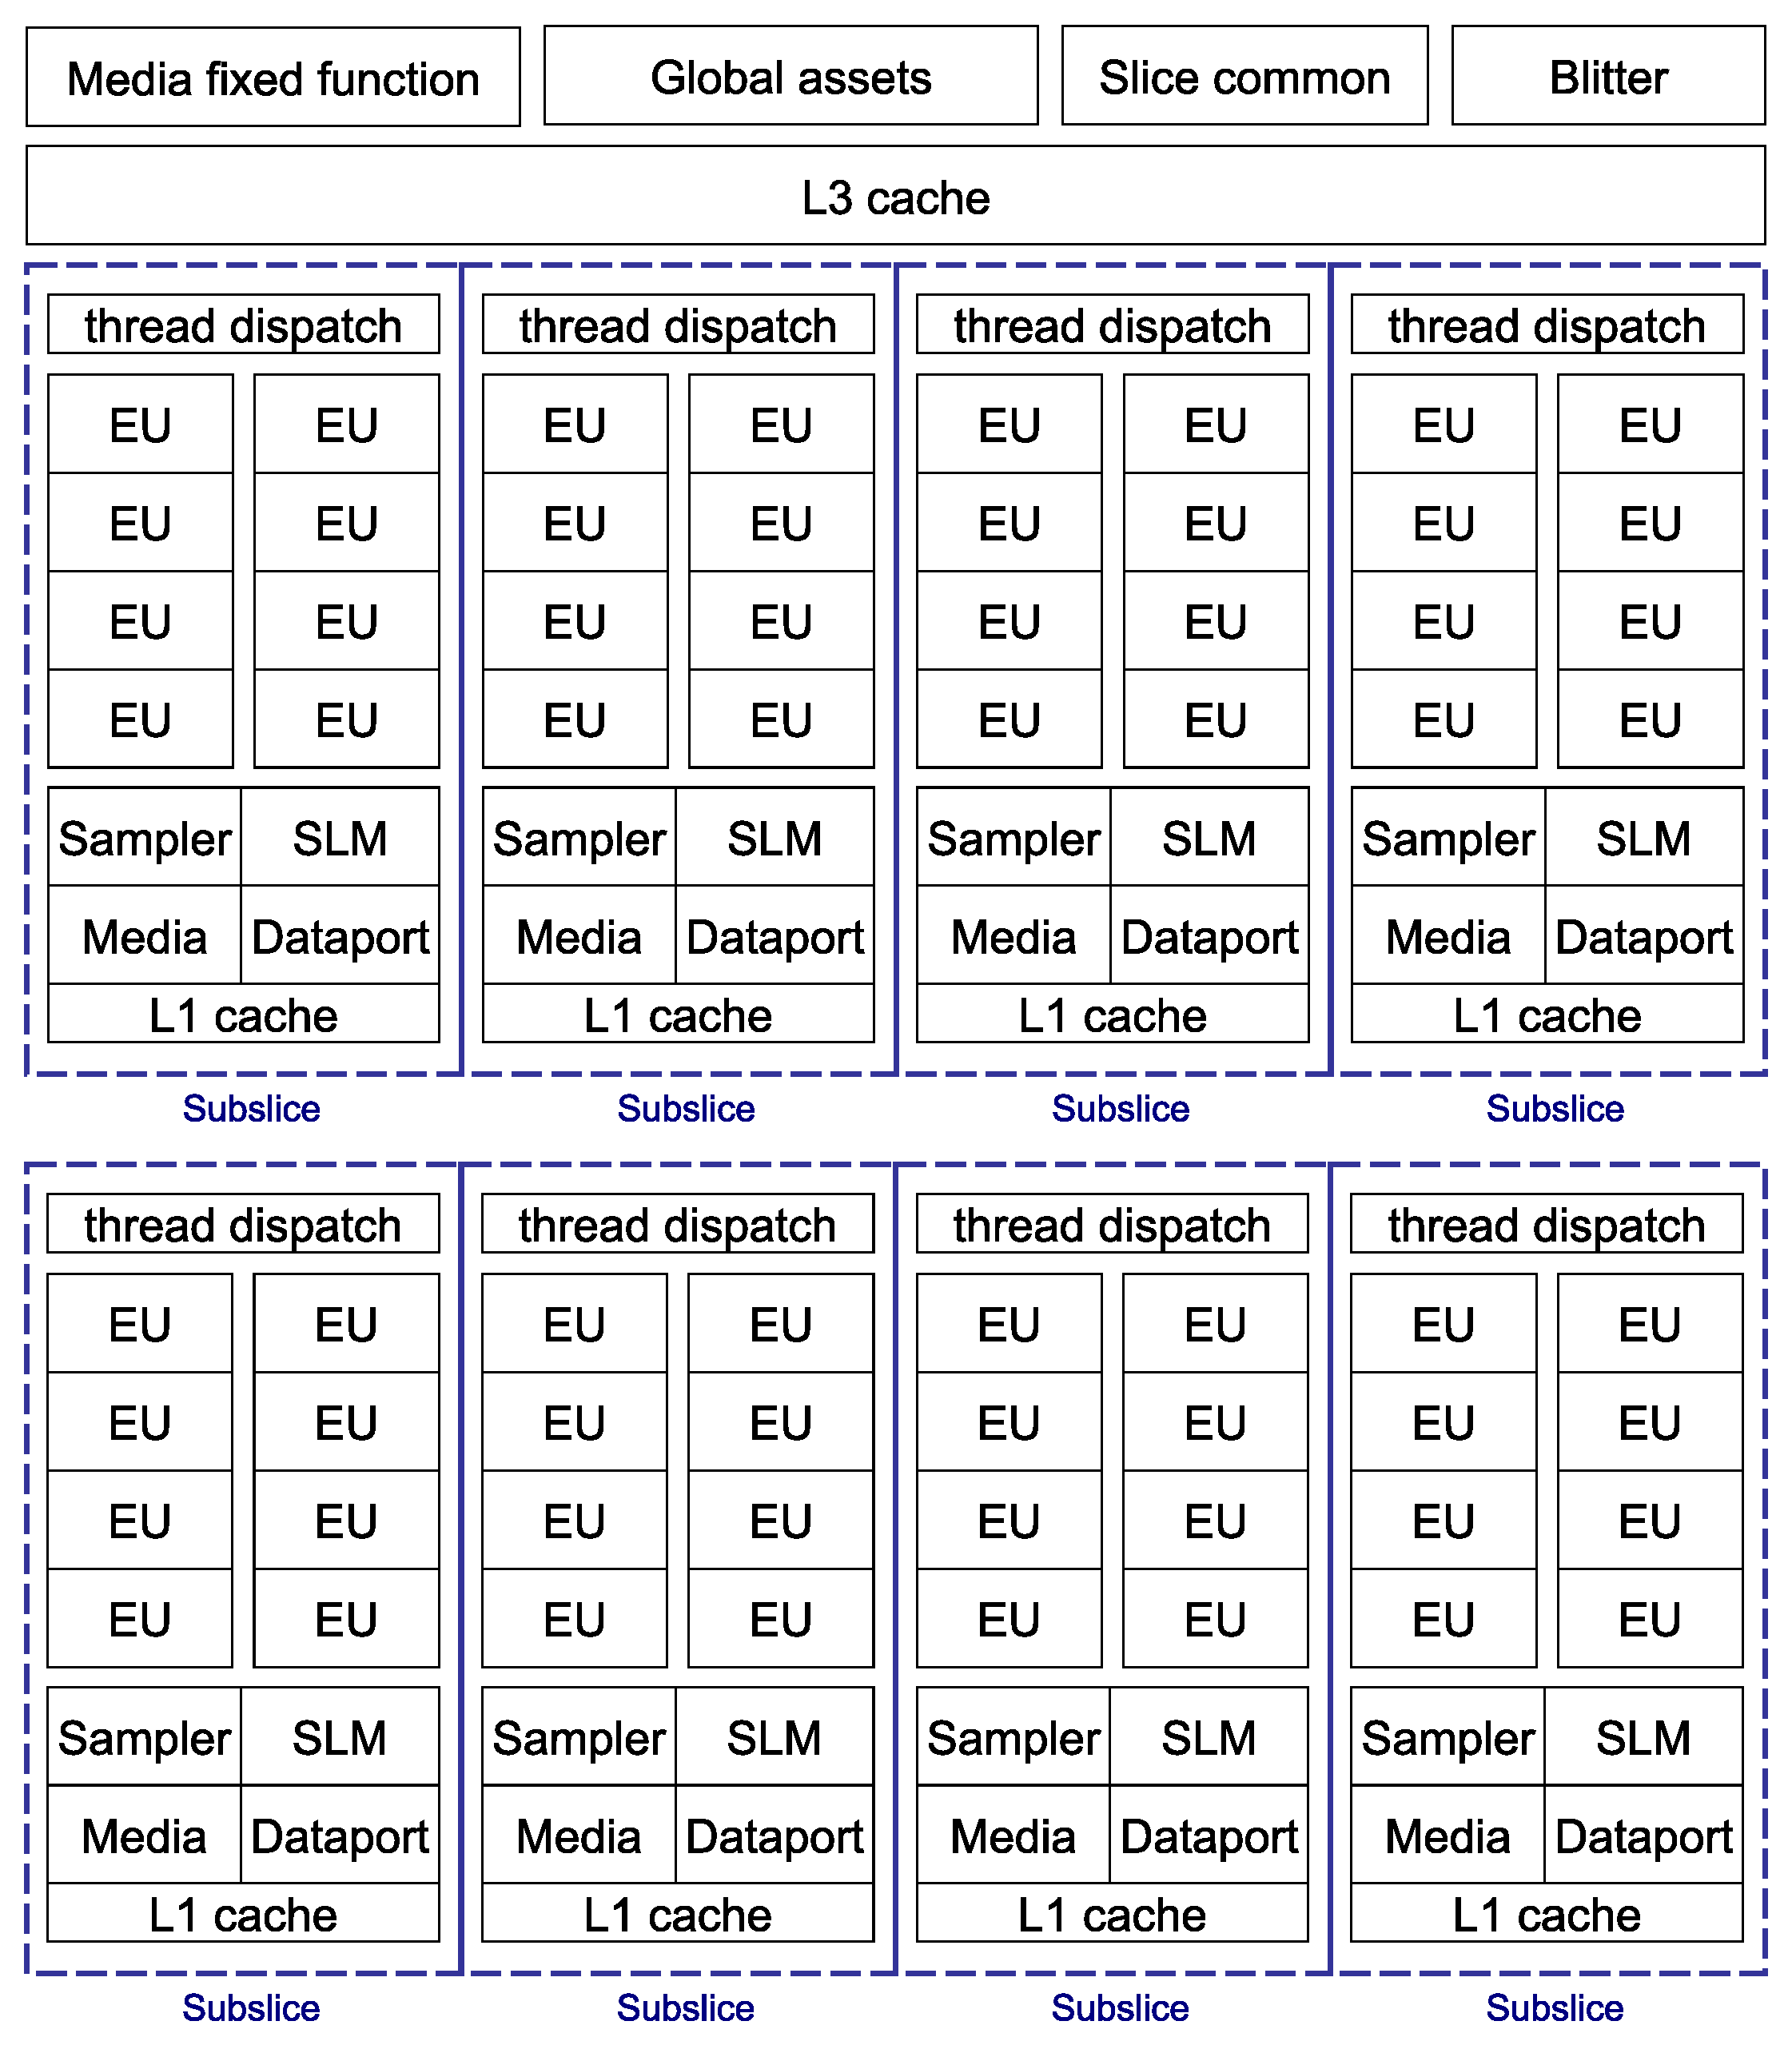
\includegraphics[scale=0.4]{Vladimirov/images/typical-GPU.pdf}
    }
    \caption{Типичное устройство GPU на примере Intel Gen 11}\label{fig:typicalGPU}
\end{figure}

Типичная современная видеокарточка (вариант Intel Gen 11) представлена на рисунке~\cref{fig:typicalGPU}. Можно видеть большое количество параллельных исполнительных устройств, у каждого из которых есть небольшой кеш первого уровня и на всех один общий кеш третьего уровня (второй уровень пропущен конструктивно). Также в каждом подслое (subslice) можно увидеть блок локальной памяти (SLM), порт для общения с глобальной памятью и некоторые фиксированные функции (медиаблок, самплер).
\nomenclature{\(SLM\)}{shared local memory, разделяемая локальная память}
\nomenclature{\(CPU\)}{central processing unit, центральный процессор}
\nomenclature{\(GPU\)}{graphics processing unit, видеокарточка}
\nomenclature{\(NPU\)}{neural processing unit, карта машинного обучения}
\nomenclature{\(API\)}{neural processing unit, карта машинного обучения}

С развитием оыбчных процессоров (CPU), количество ядер на них увеличивается. Обычно для функций контроля устройств и подготовки вычислительных задач нужно не более одного аппаратного потока. Это приводит к тому, что гетерогенная система может быть построена не только из специализированных устройств но и из свободных от функций хоста ядер хостового процессора. Такой подход называется гибридным программированием \cite{yang2017hybrid}. При таком подходе можно пересылать данные в глобальную видеопамять и инициировать гетерогенные вычисления через один интерфейс (например CUDA), а потоками хостовой машины управлять через другой интерфейс (например OpenMP). Это возможный подход к гибридной системе но конечно гораздо лучше когда вычислительная задача может быть исполнена на самых разных устройствах и все доступные устройства объединены единым интерфейсом.

На такой единый открытый интерфейс претендует, например, SYCL \cite{da2016comparative}. Есть также вариант SYCL с расширениями Intel, который называется DPC++ \cite{reinders2021dpc}. Но использование таких программных интерфейсов предполагает работу с логической моделью памяти. И здесь критически важной становится то, насколько хорошо мы оптимизируем одну и ту же программу для работы с совершенно разными устройствами. Разумеется каждое устройство имеет собственный компилятор. Например для видеоускорителей компании Intel компилятор называется Intel Graphics Compiler и он доступен публично \cite{chandrasekhar2019igc}.

Таким образом тема исследований оптимизаций в компиляторах для гетерогенных программ и в частности для графических ускорителей является актуальной. Первые публикации по этой теме начали появляться в 2000-х годах \cite{yang2010gpgpu} и тема сравнительно хорошо разработана для скалярных программных интерфейсов, например для уже упоминавшегося OpenMP \cite{lee2009openmp}. Тема которая почти не освещена в текущей литературе это работа с векторными системами команд и оптимизации памяти и потока управления для векторных программных интерфейсов. Эта работа во многом мотивирована появлением высокоуровневых векторных программных интерфейсов, таких как DPC++ESIMD и ISPC \cite{pharr2012ispc}. Язык и система программирования ISPC отлично показали себя на задачах трассировки лучей на векторных CPU, таких как процессоры Intel с расширениями AVX. Необходимость переноса этого успеха на гетерогенные и гибридные системы ставит задачу компиляции высокоуровневого векторного представления в векторную систему команд. Эта задача частично решалась графическим компилятором Intel, но как оптимальность так и функциональная корректность решения оставляли простор для исследований, особенно в части работы с памятью. Так например ранние попытки компилировать программы на ISPC для GPU показали внезапно худшую производительность чем на CPU. Эта работа адресует многие из возникших проблем и является результатом более чем трёхлетней работы автора в компании Intel и преподавания в МФТИ.

\textbf{Целью} данной работы является разработка методов и алгоритмов оптимизации работы с памятью в гетерогенных системах.

Для~достижения поставленной цели необходимо было решить следующие \textbf{задачи}:
\begin{enumerate}[beginpenalty=10000] % https://tex.stackexchange.com/a/476052/104425
  \item Разработать методологию представления высокоуровневых векторных конструкций в векторной системе команд.
  \item Разработать алгоритм разбиения структур данных для улучшения векторизации.
  \item Разработать алгоритм восстановления векторного потока управления.
\end{enumerate}

\textbf{Объектом исследования} является работа с памятью и потоком управления в гетерогенных системах.

\textbf{Предметом исследования} являются оптимизации в компиляторах для гетерогенных систем.

\textbf{Научная новизна:} 
\begin{enumerate}[beginpenalty=10000]
  \item В диссертационной работе был разработан новый метод ступенчатого понижения промежуточного представления до векторных регионов.
  \item Был разработан новый эффективный алгоритм поэлементного разбиения вложенных структур для улучшения векторизации.
  \item Было разработано предикатное представление векторного потока управления в высокоуровневом промежуточном представлении и алгоритм его восстановления на уровне работы с регионами.
\end{enumerate}

\textbf{Практическая значимость} диссертационной работы заключается в разработанном методе ступенчатого понижения промежуточного представления, алгоритме разбиения структур и алгоритме восстановления векторного потока управления.

Все разработанные методы и алгоритмы были использованы в Intel Graphics Compiler. Разработанные методы и алгоритмы позволили получить существенный прирост производительности на целевых приложениях.

Результаты работы также внедрены в кафедральный курс «Обобщённое программирование» кафедры микропроцессорных технологий в интеллектуальных системах управления МФТИ.

\textbf{Методология и методы исследования} основываются на базовых принципах системного анализа, правилах проектирования программного обеспечения, теории алгоритмов и теории графов и оптимизации.

\textbf{Основные положения выносимые на защиту:}
\begin{enumerate}[beginpenalty=10000]
  \item Метод ступенчатого понижения промежуточного представления до векторных регионов. Заключается в добавлении в конвейер оптимизации компилятора для гетерогенной системы шести обязательных и четырёх оптимизационных пассов для работы с памятью и представлением потока управления.
  \item Представления векторного потока управления в высокоуровневом промежуточном представлении 
  \item Алгоритм восстановления векторного потока управления на уровне работы с регионами.
  \item Алгоритм поэлементного разбиения вложенных структур для улучшения векторизации.
\end{enumerate}

\textbf{Достоверность} полученных результатов проверялась с помощью разработанного программного обеспечения путем замеров производительности вычислительных шейдеров на стандартных системах бенчмаркинга. Соответствие результатов необходимым целям обеспечивалось путём научно-технических консультаций с представителями отраслевой индустрии.

\textbf{Апробация работы} основные результаты работы докладывались на
\begin{itemize}
  \item семинарах ФРКТ МФТИ, 2020-2022
  \item семинарах и технических форумах в компании Intel, 2020-2021
\end{itemize}

\textbf{Личный вклад} автор заключается в:
\begin{itemize}
  \item разработке выносимых на защиту метода и алгоритмов.
  \item программной реализации ключевых компонент созданного программного обеспечения.
\end{itemize}

\textbf{Публикации}. Основные результаты по теме диссертации изложены в 2 печатных изданиях, изданых в журнале, рекомендованном ВАК.

\iffalse

% TODO: сделать vla-characteristic и сделать автореферат оттуда или просто копипаст?

\input{common/characteristic} % Характеристика работы по структуре во введении и в автореферате не отличается (ГОСТ Р 7.0.11, пункты 5.3.1 и 9.2.1), потому её загружаем из одного и того же внешнего файла, предварительно задав форму выделения некоторым параметрам

\fi

\textbf{Объем и структура работы.} Диссертация состоит из~введения,
\formbytotal{totalchapter}{глав}{ы}{}{},
заключения и
\formbytotal{totalappendix}{приложен}{ия}{ий}{}.
%% на случай ошибок оставляю исходный кусок на месте, закомментированным
%Полный объём диссертации составляет  \ref*{TotPages}~страницу
%с~\totalfigures{}~рисунками и~\totaltables{}~таблицами. Список литературы
%содержит \total{citenum}~наименований.
%
Полный объём диссертации составляет
\formbytotal{TotPages}{страниц}{у}{ы}{}, включая
\formbytotal{totalcount@figure}{рисун}{ок}{ка}{ков} и
\formbytotal{totalcount@table}{таблиц}{у}{ы}{}.
Список литературы содержит
\formbytotal{citenum}{наименован}{ие}{ия}{ий}.    % Введение
\ifnumequal{\value{contnumfig}}{1}{\counterwithout{figure}{chapter}
}{\counterwithin{figure}{chapter}}
\ifnumequal{\value{contnumtab}}{1}{\counterwithout{table}{chapter}
}{\counterwithin{table}{chapter}}
\chapter{Обзор подходов к компиляции гетерогенных приложений}\label{ch:overview}

\section{Логическое и физическое представление гетерогенных систем}\label{sec:overview/logical}

\subsection{Логическая модель памяти для GPGPU}\label{subsec:overview/logical/memory}

При работе с графическими API для вычислений (такими как OpenCL, SYCL, Cuda и прочие), программисту приходится иметь дело с несколькими уровнями памяти.
Базовое разделение это \textbf{память хоста} -- память хостовой машины, обычно это что-то вроде обычной RAM и \textbf{память устройства}, устроенная гораздо сложнее.

В обычном случае память устройства бывает следующих видов:

\begin{itemize}
\item \textbf{Глобальная} -- память на устройстве обычно большого объёма и доступная каждому EU.
\item \textbf{Виртуальная разделяемая} -- участки памяти непосредственно отображаемые на память хоста.
\item \textbf{Константная} -- память, изменение которой в программах выполняемых на устройстве запрещено.
\item \textbf{Локальная} -- память доступная только потокам внутри рабочей группы.
\item \textbf{Приватная} -- память (обычно очень небольшое её количество) доступная только конкретному EU.
\end{itemize}

Здесь бывают тонкости и нюансы в терминологии. Например память, которая в SYCL называется приватной, в CUDA называется локальной, локальная называется разделяемой, а разделяемая глобальная называется унифицированной. Но с точностью до переименований все современные программные интерфейсы работают более-менее с одной логической моделью. Далее в этой работе будет использоваться терминология SYCL.

Обычно тип памяти напрямую запрашивается при работе с программным интерфейсом как на листинге~\cref{lst:oclapi}. Такие вызовы с хоста по сути являются обращениями к графическому рантайму или как его иначе называют UMD~(user-mode driver). Он обрабатывает такого рода запросы и комбинируя их в пакеты отправляет их к нижележащему интерфейсу операционной системы.

\nomenclature{\(UMD\)}{user-mode driver, обычное название графического рантайма}
\nomenclature{\(KMD\)}{kernel-mode driver, драйвер операционной системы, требующий привилегированного исполнения}

\begin{ListingEnv}[!h]
    \captiondelim{ } 
    \caption{Пример запроса глобального буффера в OpenCL API}\label{lst:oclapi}
    \begin{lstlisting}[language={[ISO]C++}]
  cl_context Context;
  cl_mem Buf;
  cl_int Err;
  Context = clCreateContextFromType(NULL, CL_DEVICE_TYPE_GPU, NULL, 
                                    NULL, &Err);
  // .....
  Buf = clCreateBuffer(Context, CL_MEM_READ_WRITE, BUFSZ * sizeof(int), 
                       NULL, &Err);
    \end{lstlisting}
\end{ListingEnv}

Мы будем называть такого рода вызовы API-вызовами~(API call). Многие современные программные интерфейсы такие как SYCL и CUDA делают эти вызовы неявными. Другие, такие как OpenCL, наоборот, стараются делать явные вызовы. В хорошо спроектированной программе количество такого рода вызовов надо минимизировать так как такого рода общение с рантаймом не бесплатно и при неправильном использовании вносит ненужные расходы времени и памяти.

В данном случае API-вызов \lstinline!clCreateBuffer! запрашивает создание буфера в глобальной памяти. В некоторых случаях компилятор может оптимизировать работу с памятью, например сделав stateless to stateful преобразование и тогда этот буфер окажется в несколько другой памяти (при соблюдении ряда условий). Но программист всегда оперирует с логической моделью, так как это единственный способ написать общий код для нескольких устройств гибридной системы.

\begin{figure}[ht]
    \centerfloat{
        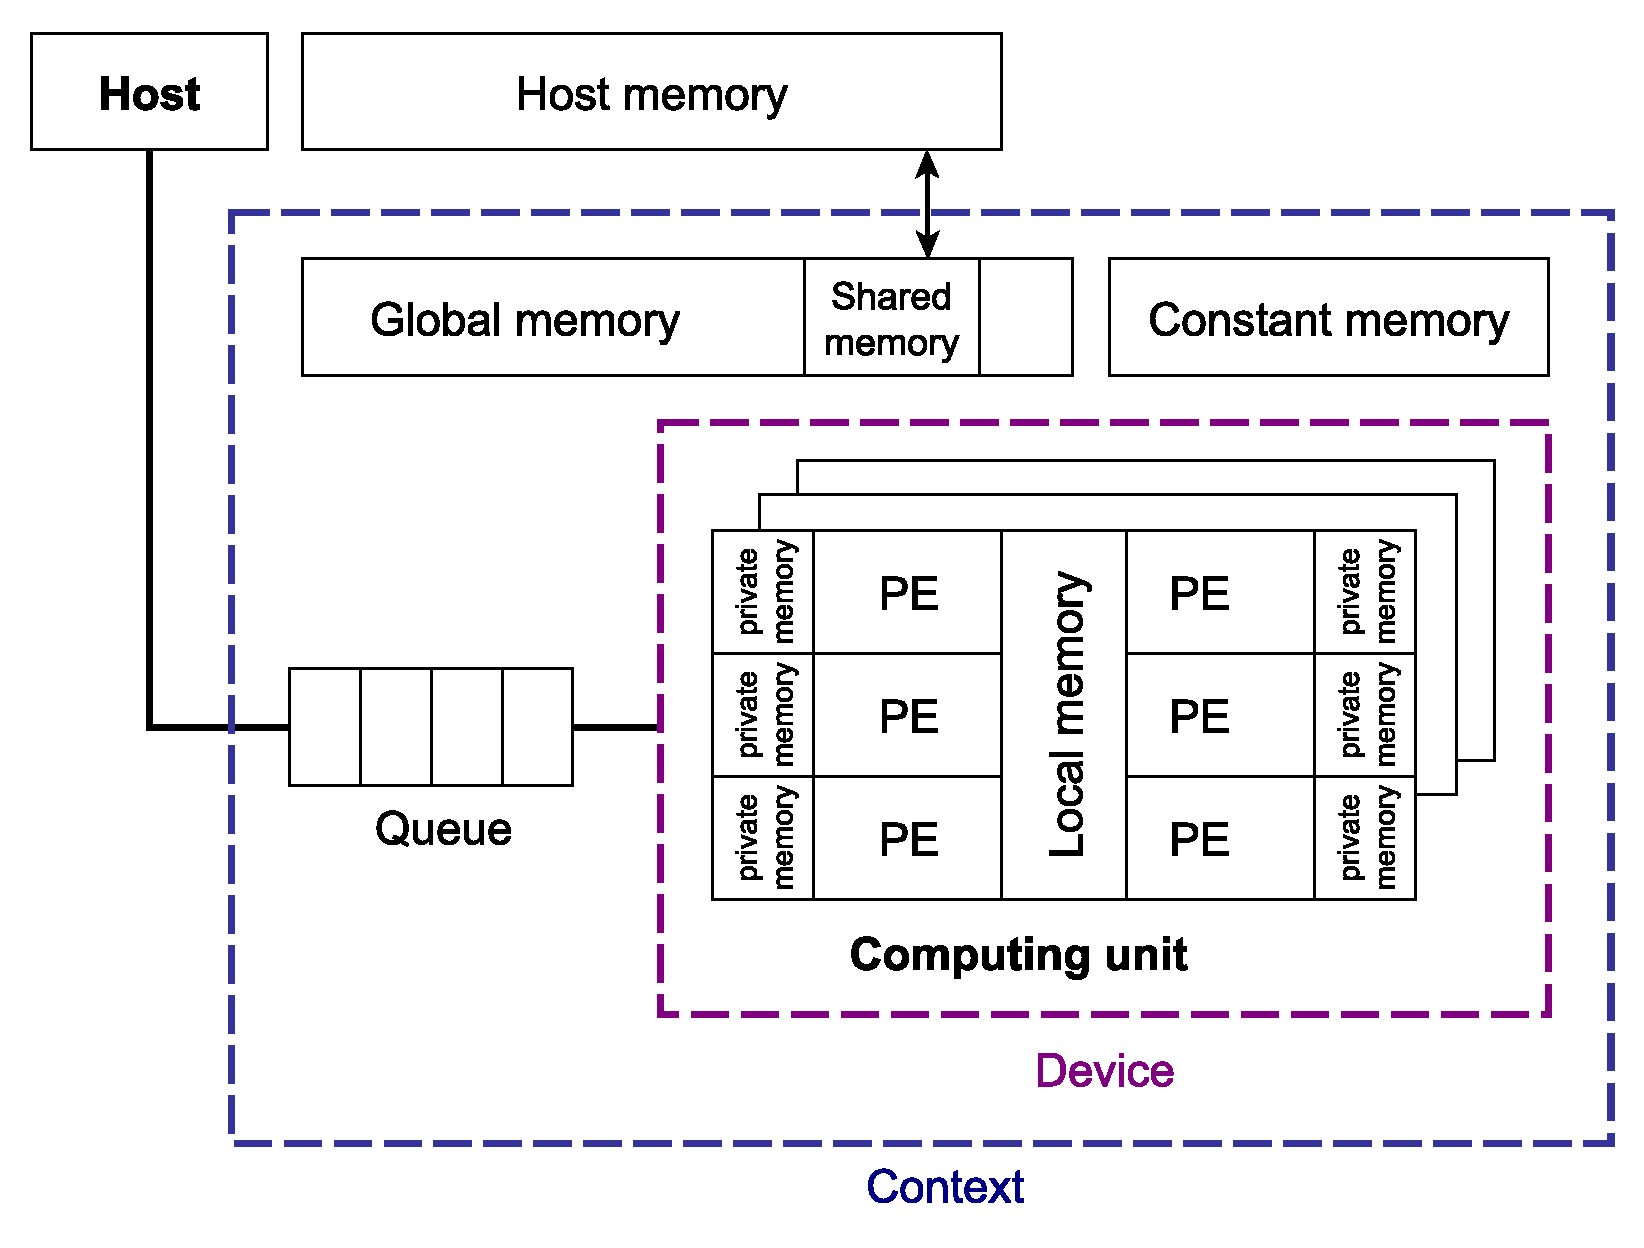
\includegraphics[scale=0.6]{Vladimirov/images/logical-memory.pdf}
    }
    \caption{Логическая модель памяти}\label{fig:logical-memory}
\end{figure}

Логическая модель памяти, характерная для таких API, как OpenCL и SYCL, представлена на рисунке~\cref{fig:logical-memory}. Ключевым понятием является computing unit (CU), комбинирующий несколько исполнительных устройств. Каждый computing unit это элемент кооперативной многозадачности внутри GPU. Все исполнительные устройства в пределах CU обладают доступом к общему пространству -- локальной памяти. Это небольшая и быстрая общая память. Она очень важна в таком виде. Но ещё важнее, что итерационное пространство рабочей группы позволяет потокам в её пределах ждать друг друга на семафорах, называемых часто барьерами.

Чтобы проиллюстрировать концепцию барьера, допустим у нас есть гнездо циклов с внутренним параллелизмом, представленное на листинге~\cref{lst:nobarrier}.

\begin{ListingEnv}[!h]
    \captiondelim{ } 
    \caption{Гнездо циклов с внутренним параллелизмом}\label{lst:nobarrier}
    \begin{lstlisting}[language={[ISO]C++}]
for (auto i : Ni)
  for (auto j : Nj)
    parallel for (auto k : Nk)
      do(i, j, k);
    \end{lstlisting}
\end{ListingEnv}

Это довольно плохой случай, так как мы можем распараллелить только самый вложенный цикл и получается, что мы должны постоянно входить в параллельное исполнение и выходить из него. Но если порядок по $k$ не важен, и $N_k$ не велико, то мы можем воспользоваться барьерами рабочей группы. Тогда это гнездо циклов трансформируется в следующий более выгодный вид, приведённый на листинге~\cref{lst:localbarrier}.

\begin{ListingEnv}[!h]
    \captiondelim{ } 
    \caption{Гнездо циклов с барьером внутри}\label{lst:localbarrier}
    \begin{lstlisting}[language={[ISO]C++}]
parallel for (auto k : Nk)
  for (auto i : Ni)
    for (auto j : Nj) {
       do(i, j, k);
       barrier(k);
    }
    \end{lstlisting}
\end{ListingEnv}

Разница в том что теперь для каждого элемента параллелизма оба дорогих вложенных цикла исполняются на своём исполнительном устройстве. Эта техника на некоторых бенчамрках, таких как перемножение матриц или битоническая сортировка позволяют выиграть до тридцати процентов производительности и более даже в простом скалярном случае.

Чтобы сделать пример более реалистичным, рассмотрим типичное гнездо циклов для практически важной задачи перемножения матриц, приведенное на листинге~\cref{lst:gemmnested}. Матрицы разбиты на тайлы и для каждого тайла мы в первом цикле запускаем копирование в локальную память и вычисление небольшого произведения в локальной памяти (мы должны помнить что она не велика). Во втором цикле мы собираем результаты обратно в глобальную память.

\begin{ListingEnv}[!h]
    \captiondelim{ } 
    \caption{Матричное перемножение с локальной памятью и вложенным параллелизмом}\label{lst:gemmnested}
    \begin{lstlisting}[language={[ISO]C++}]
private S = 0;
for (Tile = 0; Tile < NumTiles; ++Tile) {
  parallel for(auto Wi: Workitems)
    copy_global_to_local(Tile, Wi); 
  parallel for(auto Wi: Workitems)
    S = calculate_local_mmult(wi);
}
parallel for(auto Wi: Workitems)
  update_global_memory(S, Wi); 
    \end{lstlisting}
\end{ListingEnv}

Очевидно здесь внешний цикл никак не распараллелен и это приводит к существенным накладным расходам. Чтобы этого избежать, давайте формально введём барьеры и инвертируем циклы точно по той же схеме, которую мы использовали на листинге~\cref{lst:localbarrier}.

\begin{ListingEnv}[!h]
    \captiondelim{ } 
    \caption{Матричное перемножение с барьерами}\label{lst:gemmbarrier}
    \begin{lstlisting}[language={[ISO]C++}]
parallel for(auto Wi: Workitems)
  for (Tile = 0; Tile < NumTiles; ++Tile) {
    copy_global_to_local(Tile, Wi);
    barrier;
  }
parallel for(auto Wi: Workitems)
  for (Tile = 0; Tile < NumTiles; ++Tile) {
    S = calculate_local_mmult(wi);
    barrier;
  }
    \end{lstlisting}
\end{ListingEnv}

Результат такого рода инверсии приведён на листинге~\cref{lst:gemmbarrier}. Теперь мы имеем два паралелльных внешних цикла и на каждое исполнительное устройство попадает довольно большая вычислительная задача: целый внутренний цикл. Внутри него стоит барьер на котором потоки ждут друг друга в пределах локальнйо рабочей группы -- то есть собственно в пределах работы над тайлом. Внимательно глядя на оба этих цикла мы замечаем, что теперь мы внезапно можем их скомбинировать и не ждать с обновлением глобальной памяти до конца работы.

\begin{ListingEnv}[!h]
    \captiondelim{ } 
    \caption{Объединение параллельных циклов}\label{lst:gemmfinal}
    \begin{lstlisting}[language={[ISO]C++}]
parallel for(auto Wi: Workitems) {
  private S = 0;
  for (Tile = 0; Tile < NumTiles; ++Tile) {
    copy_global_to_local(Tile, Wi);
    barrier;
    S = calculate_local_mmult(wi);
    barrier;
  }
  update_global_memory(S, Wi);
}
    \end{lstlisting}
\end{ListingEnv}

Результат комбинации приведён на листинге~\cref{lst:gemmfinal}. Это довольно важная трансформация, так как мы убрали ещё одну ветку fork-join: теперь вместо того чтобы напрягать рантайм оффлоадом двух циклов, мы оффлоадим один, внутри которого ждём нужных событий на барьерах.

\subsection{Физическая модель памяти}\label{subsec:overview/logical/physmem}

Для того чтобы эффективно оптимизировать программы, работающие с памятью в пределах логической модели, компиляторы должны приниматьв  рассчёт физическое устройство памяти. Схема видеокарточки на рисунке~\cref{fig:typicalGPU} может быть обобщена, чтобы лучше показать связь между различными блоками и устройствами.

На физическом уровне память устройства делится на обладающую и не обладающую состоянием. Обладающая состоянием (stateful) память это такая память где каждый буфер имеет точку привязки (binding point) и есть поддержка в железе для быстрого преобразования binding table index (BTI) и смещения в буфере в физический адрес. У каждой адресации массива есть незримое состояние: для каждого индекса BTI есть реальный физический адрес куда отображена память и размер буфера по этому адресу, а иногда и нечто другое. Работа со stateful памятью за счёт аппаратной поддержки может быть очень эффективна, но фактически сырые (то есть stateless) указатели в такой модели оказываются запрещены: они позволяют слишком много.

\begin{ListingEnv}[!h]
    \captiondelim{ } 
    \caption{Типичная программа на GLSL для Vulkan}\label{lst:typicalvulkan}
    \begin{lstlisting}[language={[ISO]C++}]
struct Particle { vec4 pos, vel; };
layout(std140, binding = 0) buffer Pos {
  Particle particles[];
};
layout (binding = 1) uniform UBO {
  float deltaT;
  int count;
} ubo;

// ....

for (int i = 0; i < ubo.count; i += DataSz)
  if (i + x < ubo.count)
    someData[x] = particles[i + x].pos;
    \end{lstlisting}
\end{ListingEnv}

На листинге~\cref{lst:typicalvulkan} приведена типичная программа на GLSL, фрагмент взят из симуляции системы частиц~\cite{gunadi2018real}. Мы видим структуру для частицы, две точки привязки $binding_0$ и $binding_1$, к которым привязаны униформный буфер (UBO) и разделяемый буфер (SSBO). Показан также цикл обработки, когда координаты частиц аккумулируются в разделяемый буфер (видимо речь о вершинном шейдере). Глядя на этот код программист на C++ мог бы подумать что речь в целом просто об операциях с массивами и указателями.

\nomenclature{\(UBO\)}{unified buffer object, буфер в графических API для представления небольших данных}
\nomenclature{\(SSBO\)}{shared buffer object, большой буфер в грфаических API, часто отображённый на глобальную память хоста}

\begin{ListingEnv}[!h]
  \captiondelim{ } 
  \caption{Пример недопустимых операций на GLSL}\label{lst:fakepointers}
  \begin{lstlisting}[language={[ISO]C++}]
int *uboPtr = &ubo.deltaT;
int *ssboPtr = &particles[i + x].pos;
int *somePtr = CTUnknownCondition() ? ssboPtr : uboPtr;
*somePtr = 8;
  \end{lstlisting}
\end{ListingEnv}

Листинг~\cref{lst:fakepointers} разоблачает эту иллюзию. Практически все показанные на нём операции не являются легальными! Мы не можем взять указатель на объект внутри буфера так как если бы мы могли, то мы могли бы и смешать эти указатели в операции над указателями, то есть стереть информацию о точке привязки. И в этом случае у графического рантайма настали бы тяжёлые времена: ему бы потребовалось разрешать чем же всё-таки является \lstinline!somePtr!.

Локальная память фактически является обладающей состоянием, так как в локальной памяти у нас есть её условное начало и размер, но нет сквозной адресации с глобальной памятью устройства и нет возможности отображать её на память хоста. Интересно, что stateful память это классика именно графических программных интерфейсов -- и OpenGL \cite{kessenich2016opengl} и Vulkan \cite{sellers2016vulkan} работают исключительно с ней, так как это эффективно с точки зрения аппаратного ускорения и хорошо ложится на задачи рендеринга и обработки изображений. Разумеется когда появляется необходимость отображать память с хостовой машины, где никаких точек привязки уже нет, а, напротив, есть такие вещи как указатели и даже динамические структуры, состоящие из указателей, требуется более сложная память, напоминающая память хоста. Именно тут проходит важный водораздел между графикой и вычислениями на GPU.

\begin{figure}[ht]
  \centerfloat{
    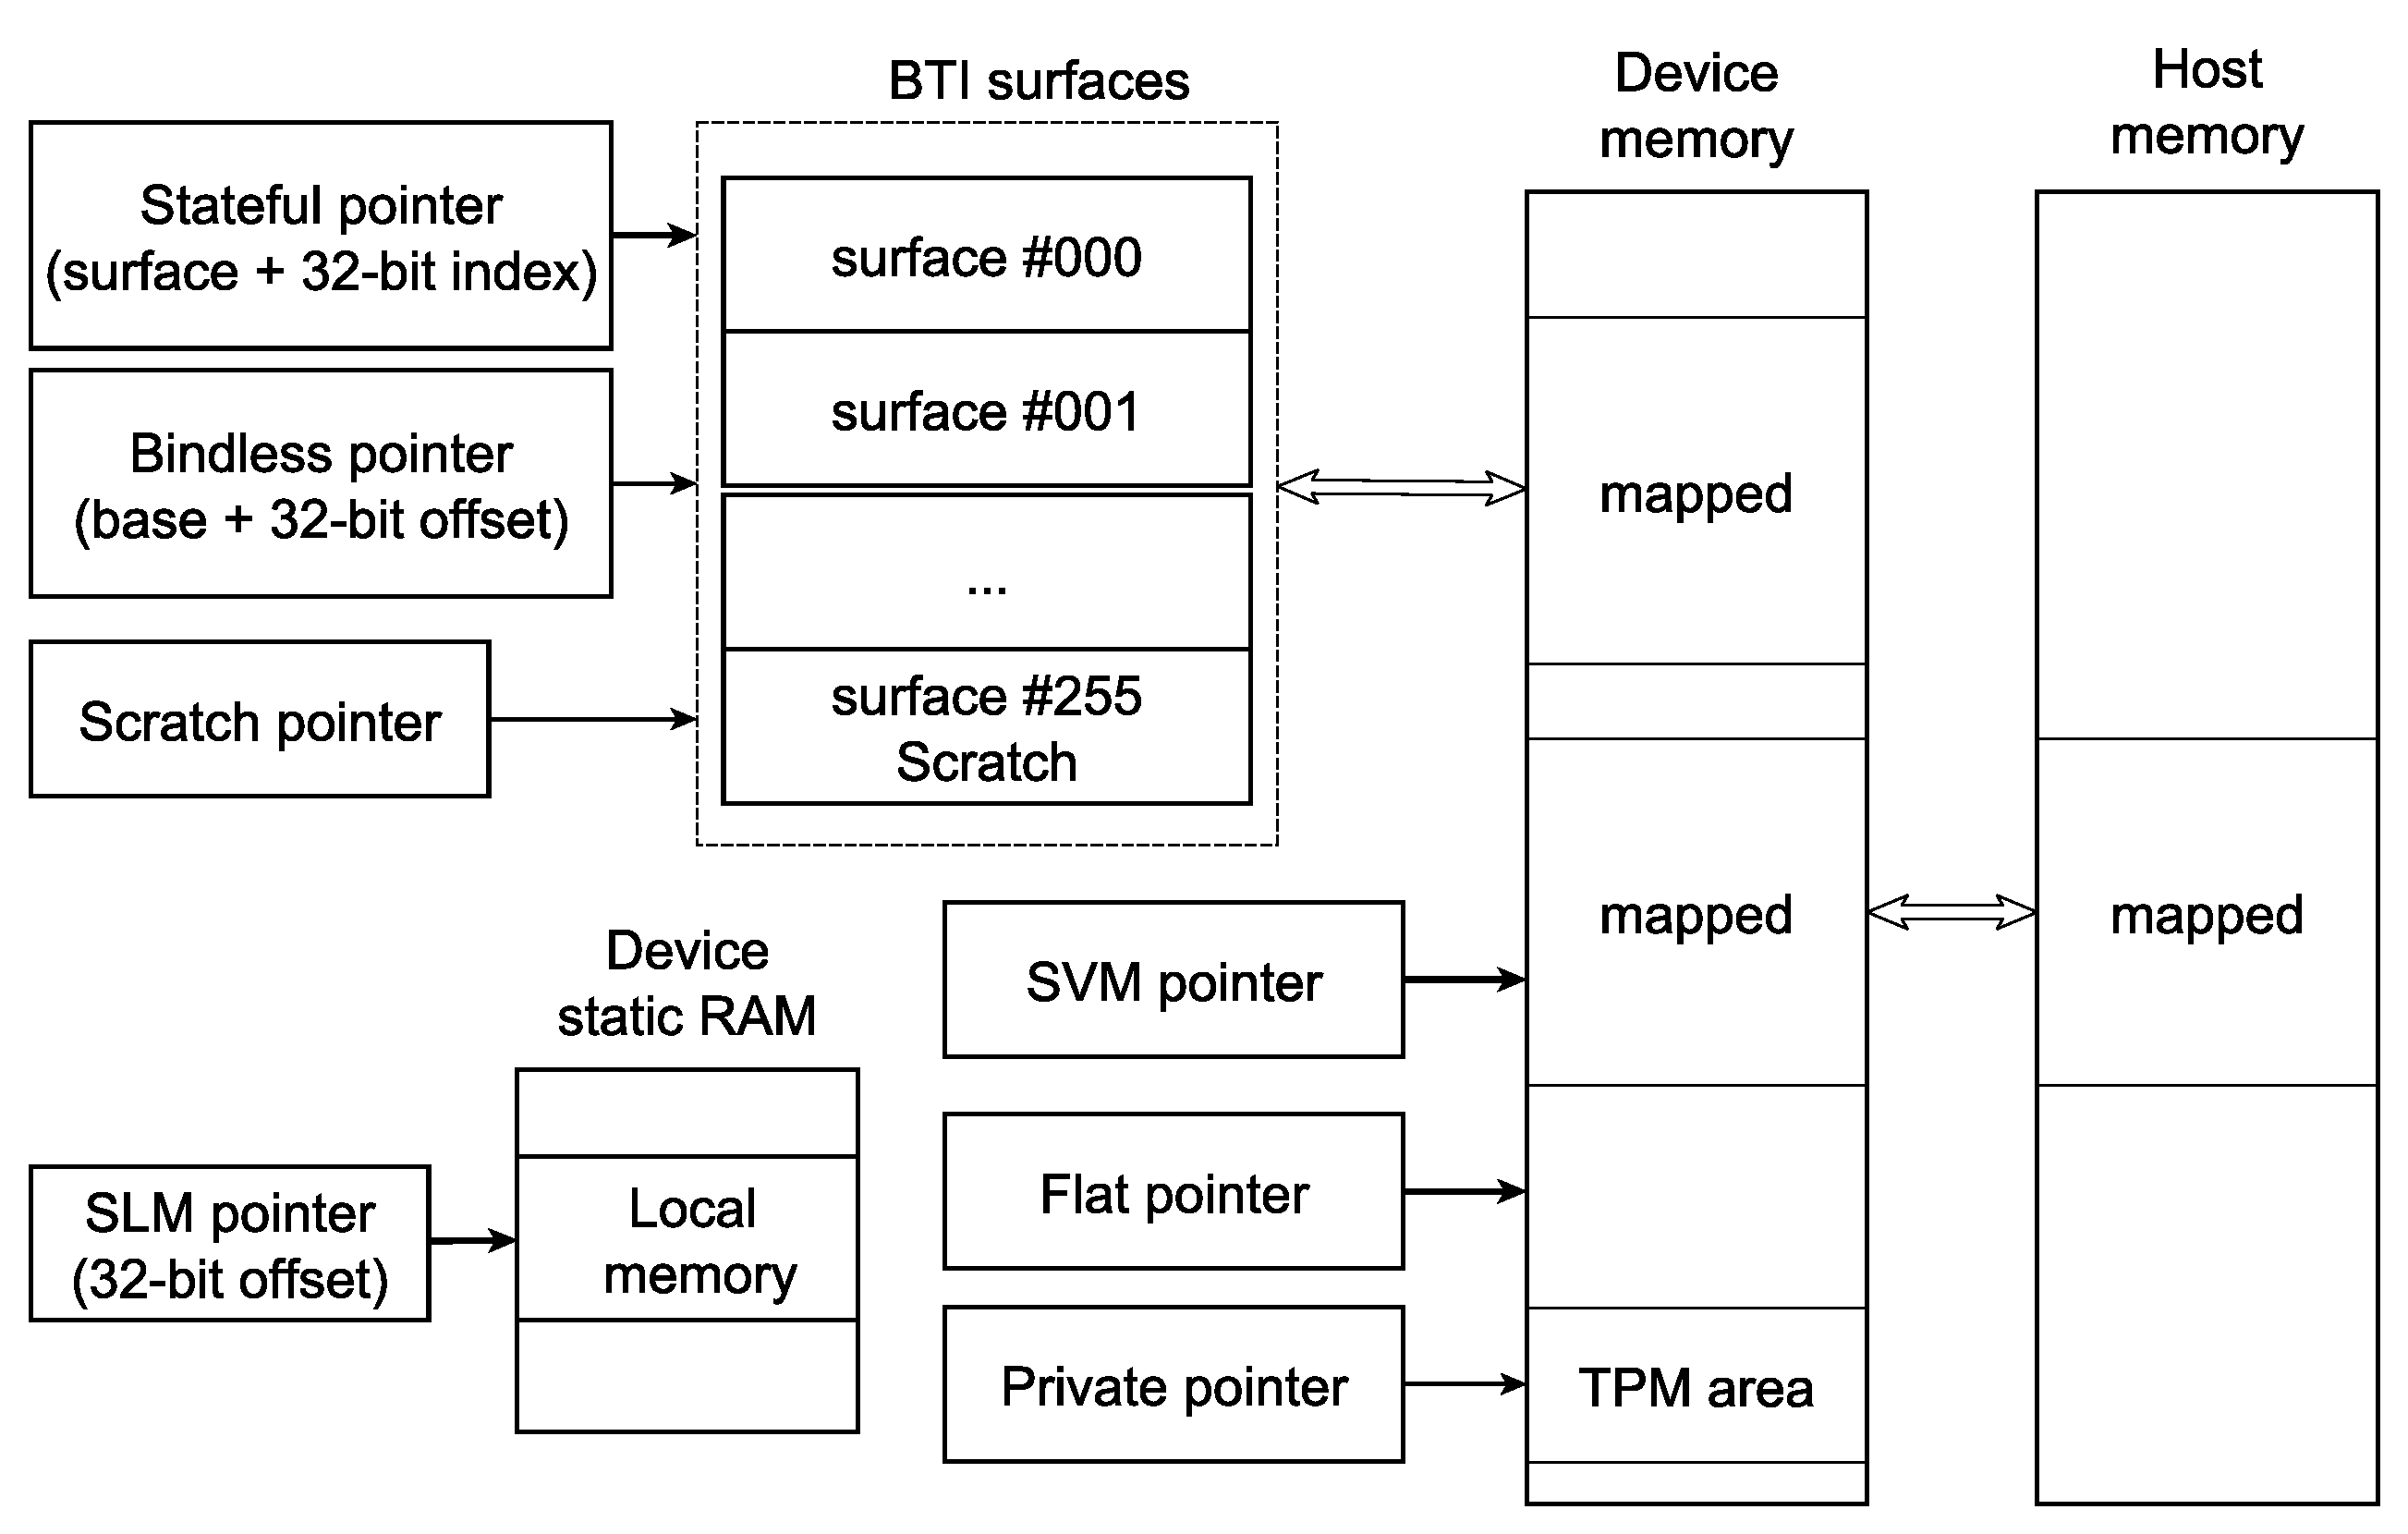
\includegraphics[scale=0.4]{Vladimirov/images/memory-scheme.pdf}
  }
  \caption{Схема физической памяти}\label{fig:memory-scheme}
\end{figure}

На рисунке~\ref{fig:memory-scheme} изображена реалистичная схема физической памяти. Локальная память показана отдельно, так как по сути это кусок L1 кеша на каждом computing unit. Собственно о локальной памяти и можно думать как о своего рода кеше.

Интересно, что само наличие памяти обладающей состоянием является для вычислительных программных интерфейсов в основном прозрачным. Компилятор часто может сделать stateless to stateful преобразование, если он может доказать, что работа ведётся в пределах одного буфера. С другой стороны известно, что сложные модели памяти часто делают компиляторные оптимизации затруднительными или невозможными \cite{vafeiadis2015common}.

Интересной концепцией является приватная память. То о чём программист на высокоуровневом графическом или вычислительном API думает как о единой сущности: небольшом и быстром пространстве для сохранения промежуточных переменных внутри шейдера, как это видно из рисунка~\ref{fig:memory-scheme}, распадается на две части: действительно небольшой и быстрый регистровый файл и кусок собственно приватной памяти, выделяемой как часть глобальной памяти (и поэтому не особо быстродействующей даже в сравнении с локальной).

\subsection{Векторный характер графических систем команд}\label{subsec:overview/logical/hw}

Все гетерогенные вычисления нужны в основном затем, чтобы максимизировать производительность.
Для этих целей в средней видеокарточке используемой в гетерогенных системах обычно просто нет операционной системы -- её драйвер это драйвер операционной системы хоста.
В связи с эти для таких устройств (это верно и для GPU и для NPU) характерно:

\begin{enumerate}
\item Отсутствие накладных расходов на переключение контекста (нет OS).
\item Сравнительно далёкая и дорогая глобальная память.
\item Часто отсутствие кешей и короткий конвейер.
\end{enumerate}

Всё это мотивирует большие регистровые файлы. Например в графических ускорителях семейства XeHPC компании Intel размер регистра может достигать 256 бит, что позволяет сохранить в одно регистре 16 целых чисел (и это не предел).

\begin{figure}[ht]
    \centerfloat{
        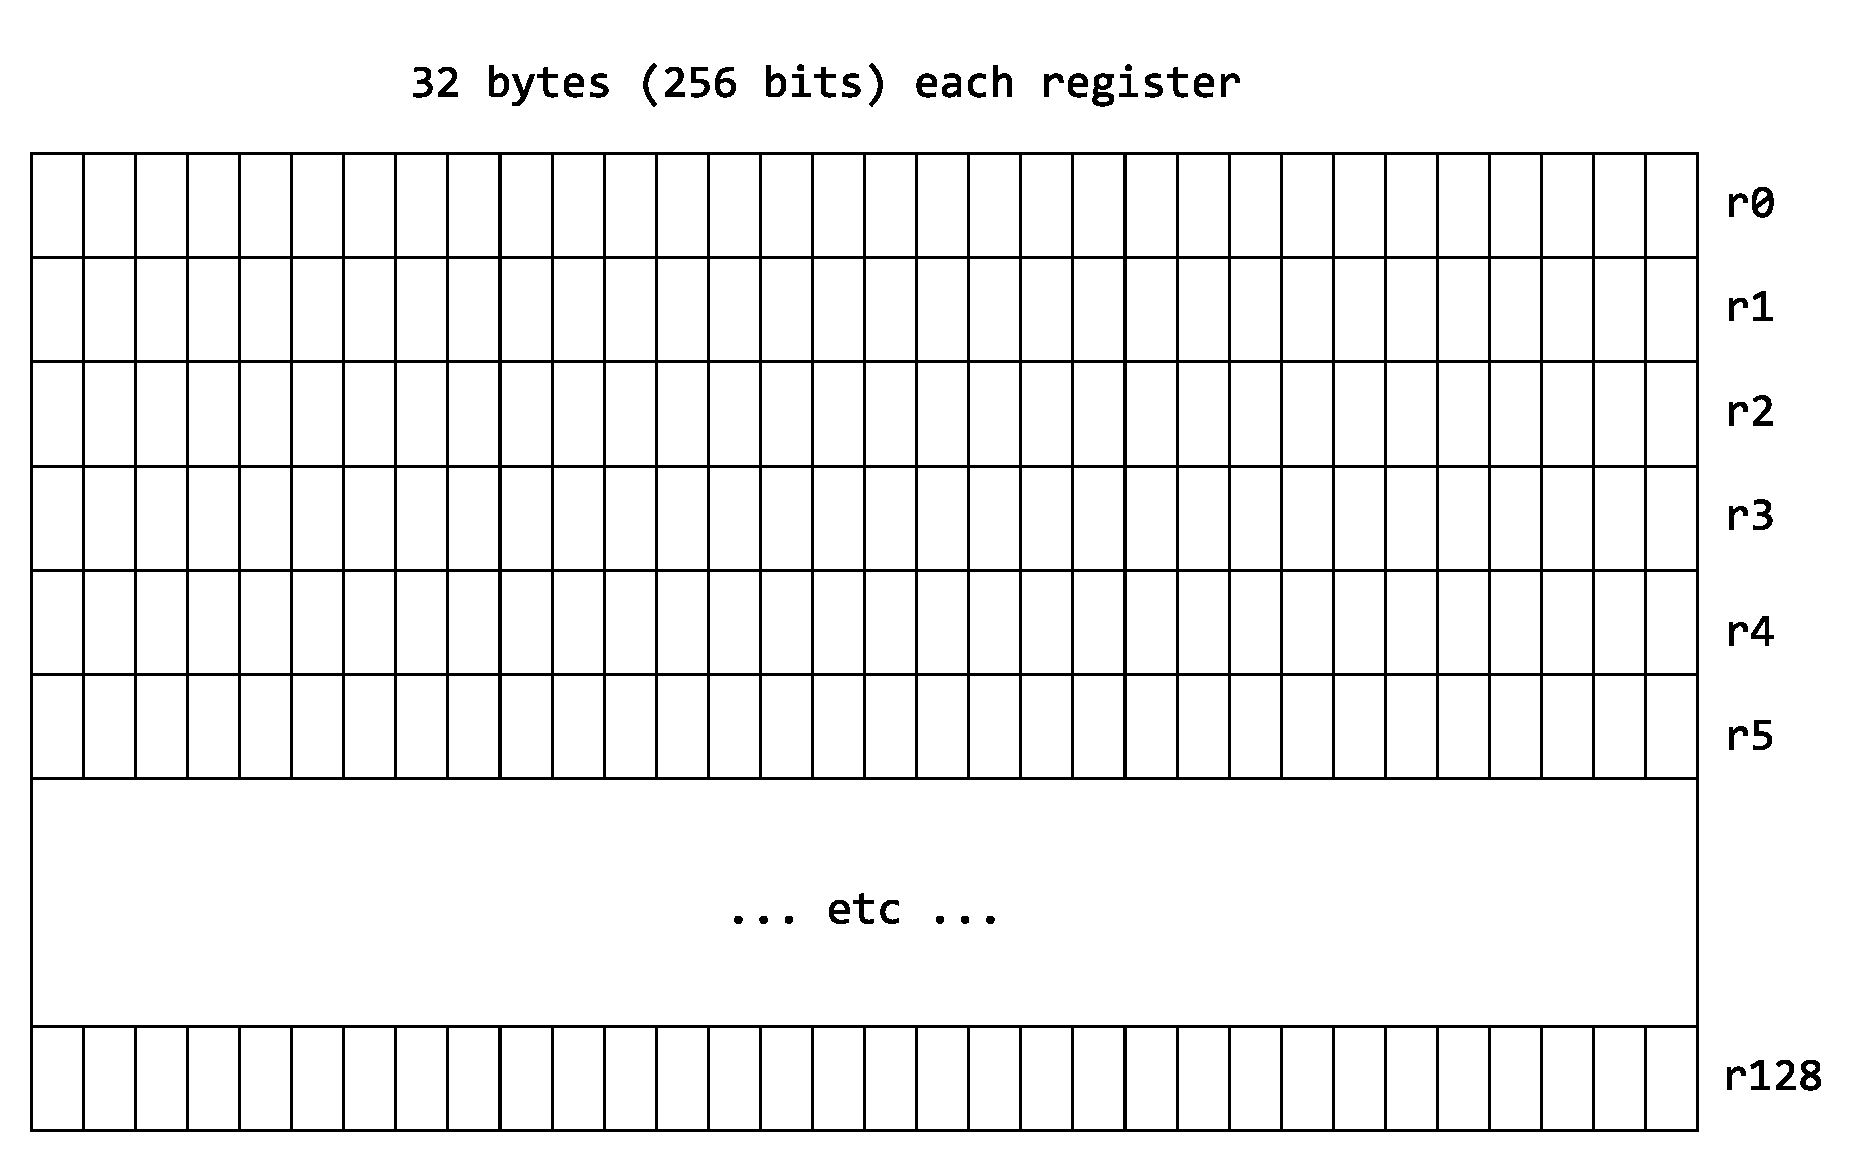
\includegraphics[scale=0.6]{Vladimirov/images/genisa-addressing-base.pdf}
    }
    \caption{Схема регистрового файла}\label{fig:genisa-addressing-base}
\end{figure}

Схема регистрового файла для архитектуры Intel XE представлена на рисунке~\cref{fig:genisa-addressing-base}. Вовсе не всегда работа с большими регистровыми файлами удобна. В программе (особенно написанной на SIMT языке) может быть расхождение управления во внутреннем цикле, могут быть разного рода нерегулярности по данным или по управляющим конструкциям которые мешают векторизации. Немного помогает подключение векторных управляющих конструкций.

\subsection{Векторный поток управления}\label{subsec:overview/logical/simdcf}

В графических ускорителях многих производителей есть возможность использовать векторный поток управления без сведения его к скалярному случаю. В архитектуре Intel Xe это реализовано через две команды: \texttt{goto} и \texttt{join}. Особенностью команды \texttt{goto} является возможность ее предикатирования. В этом случае исполнение программы произойдет так, что для предикатированных элементов вектора произойдет переход по указанной метке, а для всех остальных элементов произойдет переход на следующую инструкцию. Команда \texttt{join} восстанавливает поток управления.

В аппаратуре подобная модель исполнения реализуется с помощью маски исполнения (\textit{англ. execution mask}). Каждый бит этой маски соответствует элементу вектора. Если бит установлен в 0, то для соответствующего элемента вычисления не производятся, если же бит установлен в 1, то для соответствующего элемента исполнение происходит в обычном режиме. В самом начале программы маска состоит из единиц. Изменения в маске производят инструкции \texttt{goto} и \texttt{join}. Команда \texttt{goto} устанавливает в соответствии с предикатом биты маски в 0, выключая линии вектора, для которых условие не выполняется. Команда \texttt{join} восстанавливает маску до того состояния, в котором она находилась до изменения соответствующим \texttt{goto}.

\begin{ListingEnv}[!h]
    \captiondelim{ } 
    \caption{Пример векторного потока управления}\label{lst:simdcf}
    \begin{Verb}
  ...
  (W)     cmp  (8|M0)  (gt)f0.0  null<1>:d  r2.0<8;8,1>:d -1:w
  (~f0.0) goto (8|M0)            BB_3
  BB_1:
  (W)     add  (8|M0)            r3.0<1>:d  r2.0<8;8,1>:d  1:w
  (f0.0)  goto (8|M0)            BB_5
  BB_2:
          join (8|M0)            BB_3
  BB_3:
          add  (8|M0)            r3.0<1>:d  r2.0<8;8,1>:d -1:w
  BB_4:
          join (8|M0)            BB_5
  BB_5:
  ...
    \end{Verb}
\end{ListingEnv}

На листинге~\cref{lst:oclapi}. пример кода c векторным потоком управления на языке ассемблера для архитектуры графических ускорителей Intel. В данном примере реализовано проверка того, что в регистре r2 лежит значение большее, чем -1, а результат сравнения записан во флаговый регистр f0. Далее следует предикатированный регистром f0 условный переход: если условие для данной линии исполнения выполняется, то не происходит переход в базовый блок BB3, и к данным элементам прибавляется 1, а результат записывается в регистр r3. Для других элементов следует переход в базовый блок BB3, где из остальных элементов вычитается 1, а результат так же записывается в регистр r3.

\begin{figure}[ht]
    \centerfloat{
        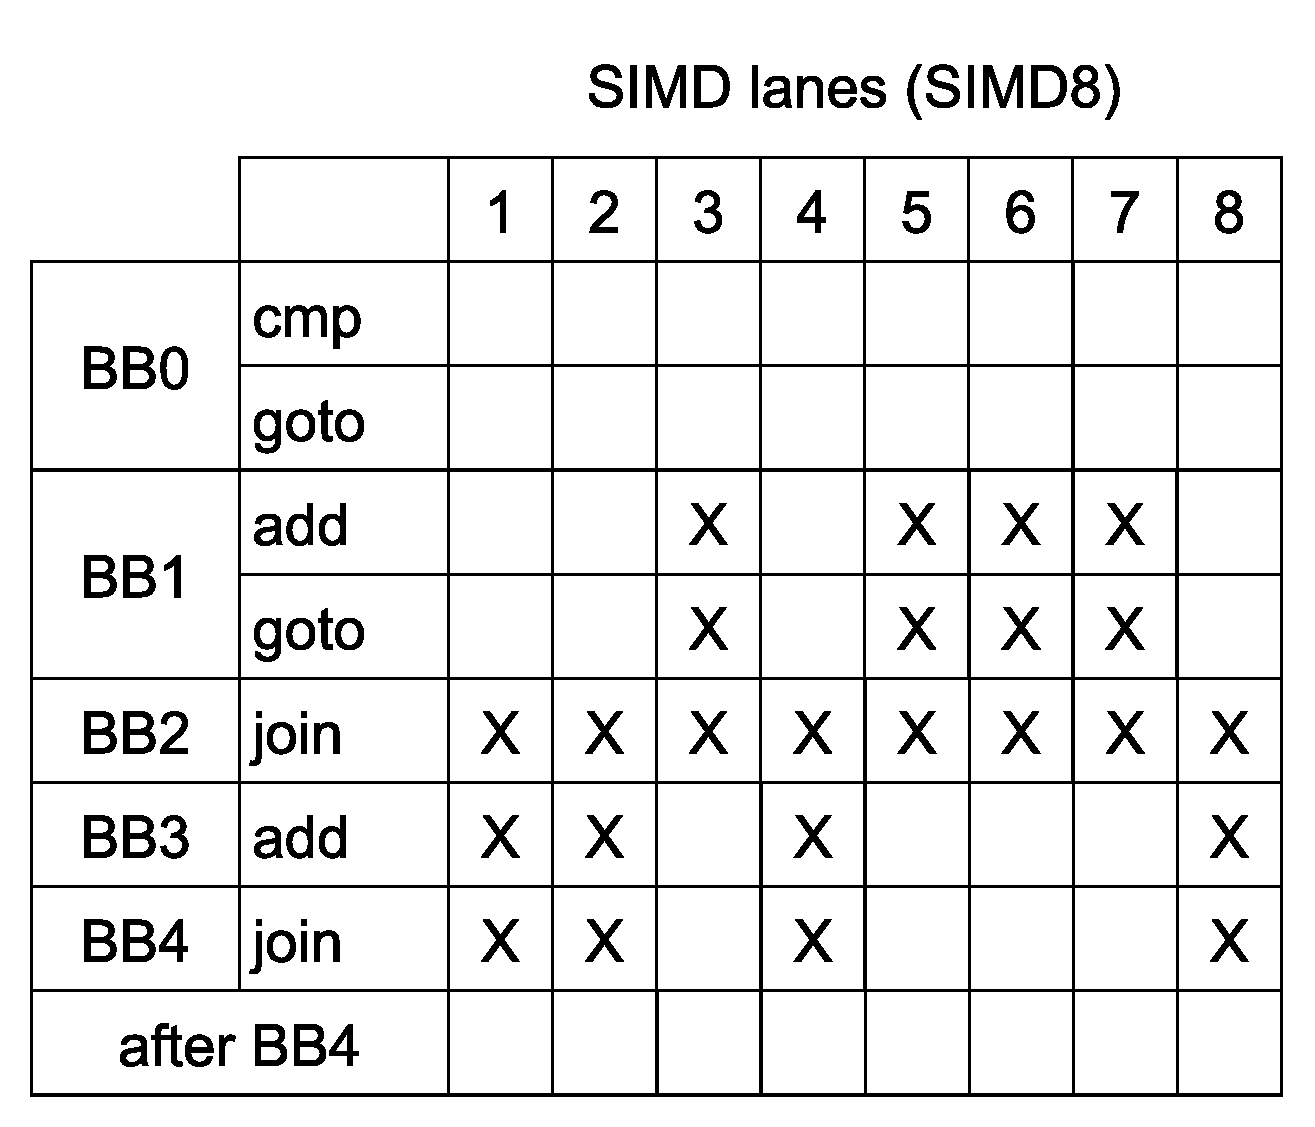
\includegraphics[scale=0.5]{Vladimirov/images/HW-goto-example.pdf}
    }
    \caption{Схема векторного потока управления}\label{fig:HW-goto-example}
\end{figure}

На рисунке~\ref{fig:HW-goto-example} схематично изображено, как будет происходить исполнение данного кода. Цифрами сверху обозначены номера линий исполнения в SIMD АЛУ, зеленым обозначены включенные линии, после исполнения предшествовавшей инструкции, а оранжевым -- выключенные.

\section{Высокоуровневые векторные интерфейсы}\label{sec:overview/vectorapi}

\subsection{ISPC}\label{subsec:overview/vectorapi/ispc}

Язык программирования и система компиляции ISPC (Intel SPMD Program Compiler) построенf для компиляции высокопроизводительного кода для гибридных систем. Изначально система была ориентирована в основном на CPU, но её концепции не менее эффективно могут быть представлены для современных GPU. Система построена так, чтобы масштабироваться как с ростом колчиества доступных ядер так и с увеличением доступной ширины векторов, легко интегрироваться в различные вычислительные окружения.

ISPC возник и до сих пор активно применяется для написания систем программной трассировки лучей \cite{moreau2019dynamic}. Изначально он был ориентирован на CPU \cite{pharr2013ray} в частности на расширения AVX512, но язык и сама модель SPMD программирования оказались настолько удачными \cite{pharr2018guest}, что его распространение на гетерогенные векторные системы стало вопросом времени.

Как и многие системы такого рода, IPSC имеет синтаксис похожий на синтаксис языка C, но с введёнными туда новыми концепциями uniform и varying переменных. Код выглядит скалярным, но каждая varying переменная (то есть любая не объявленная как uniform) является на самом деле вектором и может принимать разные значения в разных линиях маски выполнения. Базовой varying переменной является переменная \lstinline!programIndex!.

\begin{ListingEnv}[!h]
    \captiondelim{ } 
    \caption{Пример программы на ISPC вычисляющей фрактал}\label{lst:ispcmandel}
    \begin{lstlisting}[language={[ISO]C++}]
void mandelbrot_ispc(uniform float x0, uniform float y0,
                     uniform float x1, uniform float y1,
                     uniform int width, uniform int height,
                     uniform int maxIterations,
                     uniform int output[]) {
  uniform float dx = (x1 - x0) / width, dy = (y1 - y0) / height;
  for (uniform int j = 0; j < height; j++) {
    for (uniform int i = 0; i < width; i += programCount) {
      float x = x0 + (programIndex + i) * dx;
      float y = y0 + j * dy;
      int index = j * width + i + programIndex;
      output[index] = mandel(x, y, maxIterations);
    }
  }
}
    \end{lstlisting}
\end{ListingEnv}

Пример программы на ISPC приведён на листинге~\cref{lst:ispcmandel}. Обратите внимание, что значения переменных \lstinline!x!, \lstinline!y!, \lstinline!index! на самом деле являются векторными. Это обеспечивает таким программам отличную производительность, позволяет смешивать скалярные и векторные вычисления, иметь единое когерентное пространство имён и встроенную в язык поддержку AoS и SoA.

\subsection{SYCL SIMD extensions}\label{subsec:overview/vectorapi/dpcppesimd}

ESIMD расширения в SYCL это расширения, которые позволяют для SYCL программирование с явным векторным представлением. Существовавшие до этого в SYCL подгруппы слишком сложны в обращении. Как пример, на листинге~\cref{lst:syclhisto} приведена часть реализации вычисления гистограммы на SYCL, использующая явные подгруппы.

\begin{ListingEnv}[!h]
    \captiondelim{ } 
    \caption{Вычисление гистограммы на SYCL с явными подгруппами}\label{lst:syclhisto}
    \begin{lstlisting}[language={[ISO]C++}]
for (int I = N; I < NumData / NumBins; I += NGSZ) {
  for (int J = 0; J < NumBins; J += 1) {
    const int Base = G * LSZ + SGI * SLR;
    const int Idx = I * NumBins + Base + J * SGSize;
    const auto VData = SubGroup.load(BufferData + Idx);
    for (int K = 0; K < SGSize; K++) {
      auto Y = sycl::group_broadcast(SubGroup, VData, K);
      if (SLI == (Y % SGSize))
        PrivateHist[Y / SGSize] += 1;
    \end{lstlisting}
\end{ListingEnv}

Видно что мы имитируем векторное чтение с помощью \lstinline!SubGroup.load! и формируем значение, делая векторный регистр с помощью \lstinline!sycl::group_broadcast!. Это не слишком эффективно из-за лишних броадкастов и очень сложно в написании. Гораздо проще и эффективней работать сразу с векторами.

\begin{ListingEnv}[!h]
    \captiondelim{ } 
    \caption{Работа с Explicit SIMD расширением SYCL}\label{lst:syclesimd}
    \begin{lstlisting}[language={[ISO]C++}]
constexpr unsigned VL = 16;
auto Kern = [=](sycl::id<1> Id) SYCL_ESIMD_KERNEL {
  unsigned Offset = Id * VL * sizeof(float);
  esimd::simd<T, VL> VA = esimd::block_load<T, VL>(A, Offset);
  esimd::simd<T, VL> VB = esimd::block_load<T, VL>(B, Offset);
  esimd::simd<T, VL> VC = VA + VB;
  esimd::block_store(C, Offset, VC);
};
    \end{lstlisting}
\end{ListingEnv}

На листинге~\cref{lst:syclesimd} приведён пример векторного сложения в DPC++ ESIMD. Здесь и далее под DPC++ будем понимать SYCL с некоторыми специальными расширениями \cite{reinders2021dpc}. В той же работе приведена достаточная мотивация появления таких расширений и замеры положительного эффекта на производительность. Также благодаря использованию явных векторных API для реализации приложений машинного обучения, видеокарта PVC \cite{gomes2022ponte} существенно превзошла более мощные по аппаратуре видеокарты от конкурирующих компаний на задачах inference для resnet50.

\section{Обзор существующих подходов к векторизации}\label{sec:overview/vectorizing}

Теперь когда мы познакомились с основными векторными программными интерфейсами, какзалось бы нет ничего проще чем отобразить их один в один на векторную же аппаратуру. Чтобы разоблачить это заблуждение давайте посмотрим на существующие механизмы векторизации для скалярных и векторных программных интерфейсов.

Большая часть существующих процессоров показывают пиковую производительность благодаря той или иной форме векторизованных инструкций \cite{bialas2015benchmarking}. Это верно и для CPU, например Intel XEON с расширениями AVX и для GPU. Например AMD Graphics Cores Next имеет 64-линейные вектора, а NVIDIA CUDA имеет 32-линейные варпы. Варп \cite{passerat2015warp} это специальный термин для неявного параллелизма обеспечиваемого средствами аппаратного обеспечения. По самой природе таких инструкций, все операции над вектором выполняются одновремено (по крайней мере концептуально). Это ограничивает класс алгоритмов, который может быть эффективно реализован на таких архитектурах. Разумеется цена будет разной при разных подходах.

\subsection{Скалярная ISA и скалярное API}\label{subsec:overview/vectorizing/cuda}

Модель CUDA при реализации высокоуровневой программы делает крайне лёгким написание программы в которой векторный поток управления расходится. Это кстати будет далее характерно и для OpenCL и вообще это верно для любого скалярного API, полагающегося на неявную векторизацию. Она моделирует вычислительную задачу как большое количество потоков исполняющих одну небольшую программу, называемую кернелом или шейдером и для программиста это выглядит как многопоточное параллельное исполнение (SIMT).

\begin{ListingEnv}[!h]
    \captiondelim{ } 
    \caption{Пример кернела на CUDA с замером цикла}\label{lst:cudashader}
    \begin{lstlisting}[language={[ISO]C++}]
__global__ void single_loop(int* limits, float* out) {
  int tid = blockDim.x * blockIdx.x + threadIdx.x;
  int M = limits[threadIdx.x];
  for (int k = 0; k < N_UNROLL; ++k)
    for (int i = 0; i < M; i++)
      sum += EXPR_INNER;
  __syncthreads();
  out[tid] = sum;
}
    \end{lstlisting}
\end{ListingEnv}

Фактически многие руководство CUDA Programming Guide \cite{guide2013cuda} утверждает, что для корректности программист может в целом игнорировать SIMT поведение. Однако серьёзные улучшения производительности могут быть получены если учесть, требует ли код различные потоки внутри варпа расходиться.

На архитектуре NVIDIA потоки группируются в варпы по 32 потока каждый, которые должны исполнять одни и те же инструкции по сути в векторном виде. Из этого следует, что любая инструкция, которая выполняет условный переход, не дающая одного и того же значения в пределах варпа ведёт к неявному расхождению потока управления. В статье про архитектуру Tesla \cite{lindholm2008nvidia} упомянуты механизмы, которыми аппаратура пытается справляться с этой задачей, например стек синхронизации переходов.

\subsection{Векторная ISA и скалярные интерфейсы}\label{subsec:overview/vectorizing/sycl}

Начиная с разработки OpenCL как фактического стандарта гетерогенных вычислений \cite{munshi2011opencl}, можно отсчитывать время подъёма скалярных интерфейсов. Несмотря на ограниченную поддержку в таких интерфейсах векторных типов, там нет ни возможности завести вектора произвольной длины ни поддержку сложных высокоуровневых опрераций с векторами. Скалярными строго говоря были и ранние графические интерфейсы, такие как OpenGL.

Но в отличие от графических, вычислительные интерфейсы сразу ориентировались на прозрачную (или плоскую) модель памяти, единую на хосте и устройствах. Это и другие соображения (например корректность и безопасность типов по границам вычислительного интерфейса) привели к довольно быстрому подъёму скалярных интерфейсов с совмещенным исходным кодом, например SYCL \cite{reinders2021sycl}. 

\begin{ListingEnv}[!h]
    \captiondelim{ } 
    \caption{Пример кода на SYCL}\label{lst:syclshader}
    \begin{lstlisting}[language={[ISO]C++}]
auto Evt = Q.submit([&](sycl::handler &Cgh) {
  auto A = BufA.template get_access<sycl_read>(Cgh);
  auto B = BufB.template get_access<sycl_read>(Cgh);
  auto C = BufC.template get_access<sycl_write>(Cgh);

  auto Kernmul = [=](sycl::id<2> WorkItem) {
    const int Row = WorkItem.get(0);
    const int Col = WorkItem.get(1);
    T Sum = 0;
    for (int K = 0; K < AY; K++)
      Sum += A[Row][K] * B[K][Col];
    C[Row][Col] = Sum;
  };

  Cgh.parallel_for<class mmult<T>>(Csz, Kernmul);
});
    \end{lstlisting}
\end{ListingEnv}

На листинге~\cref{lst:syclshader} приведен пример довольно наивного перемножения матриц на SYCL. Основная проблема компиляции такого рода шейдеров заключается в том, что мы всё-таки компилируем их в векторную систему команд. То есть векторизация должна быть включена как шаг оптимизационного конвейера. Скалярный компилятор \cite{weiss1987study} даёт базовые возможности такого рода, но обычно включает векторизацию после основных оптимизаций как часть кодогенерации. Это логично вытекает из простого соображения: скалярный компилятор не способен оптимизировать векторный код, значит логично сначала оптимизировать, потом векторизовать.

Это создаёт различные проблемы. Наиболее известны проблемы с векторизацией внешних циклов \cite{vasudevan1982inner}. Ещё более существенной проблемой является влияние на распределение регистров. По разному автовекторизованный код вызывает разное регистровое давление. Из-за этого векторизация вынужденно включается в цикл попыток векторизации и распределения регистров, также люди изобретают различные эвристики и прочее. то есть с одного и того же кода мы можем получить как итоговый ассемблер векторизованный на максимальную ширину (например на $16$) так и на ширину поменьше но более выгодную с точки зрения распределителя (например на $8$). Это называется SIMDX-dispatch и хуже всего в нём то, что он находится вне контроля программиста. 

Таким образом упражнения на программирование в скалярном интерфейсе с векторной системой команд это почти всегда упражнение на подчинение своего рода волшебства. Программист никогда не знает приведут ли небольшеи изменения его кода к небольшим изменениям производительности или к огромным.

Большим шагом вперёд в развитии языка SYCL стал момент, когда им заинтересовалась компания Intel в рамках развития инцииативы OneAPI. Количество и качество предложенных в SYCL расширений оказалось таковым, что фактически сформировало новый язык DPC++ \cite{ashbaugh2020data}, впрочем в последнее время от этого названия уходят по мере того как новые и новые специфичные расширения становятся частью языка SYCL. Интерес к OneAPI также подогревается тем фактом, что она с одной стороны не зависит от вендора, а с другой стороны предоставляет достаточно возможностей для портирования шейдерного кода с проприетарных систем, например с CUDA \cite{christgau2020porting}.

\subsection{Векторное API с ручным управлением регистровым файлом}\label{subsec:overview/vectorizing/cm}

Для решения проблемы воспроизводимой производительности, обозначенной в \cref{subsec:overview/vectorizing/sycl} был разработан язык C for Media (он же C for Metal или просто CM). CM (C-for-Metal) \cite{lueh2021c} -- язык программирования, являющийся расширением С++ и явно реализующий концепцию SIMD. CM является языком с раздельным исходным кодом, то есть компиляция кода хоста и кода устройства происходит раздельно. На данный момент целевыми являются только архитектуры графических ускорителей Intel, но спецификация CM не является проприетарной.

\begin{ListingEnv}[!h]
    \captiondelim{ } 
    \caption{Пример кода на CM}\label{lst:cmshader}
    \begin{lstlisting}[language={[ISO]C++}]
template <typename T>
CM_NODEBUG _GENX_ inline void
transpose_matrix(matrix_ref<T, 8, 8> m1, matrix_ref<T, 8, 8> m2) {
    // 32 bit mask to control how to merge two vectors.
    uint32_t mask = 0x55555555;
    matrix_ref<T, 4, 16> t1 = m1.format<T, 4, 16>();
    matrix_ref<T, 4, 16> t2 = m2.format<T, 4, 16>();

    // j = 1
    t2.row(0).merge(t1.replicate<8, 1, 2, 0>(0, 0), 
                    t1.replicate<8, 1, 2, 0>(2, 0), mask);
    t2.row(1).merge(t1.replicate<8, 1, 2, 0>(0, 8), 
                    t1.replicate<8, 1, 2, 0>(2, 8), mask);
    t2.row(2).merge(t1.replicate<8, 1, 2, 0>(1, 0), 
                    t1.replicate<8, 1, 2, 0>(3, 0), mask);
    t2.row(3).merge(t1.replicate<8, 1, 2, 0>(1, 8), 
                    t1.replicate<8, 1, 2, 0>(3, 8), mask);

    // j = 2
    t1.row(0).merge(t2.replicate<8, 1, 2, 0>(0, 0), 
                    t2.replicate<8, 1, 2, 0>(2, 0), mask);
    t1.row(1).merge(t2.replicate<8, 1, 2, 0>(0, 8), 
                    t2.replicate<8, 1, 2, 0>(2, 8), mask);
    t1.row(2).merge(t2.replicate<8, 1, 2, 0>(1, 0),
                    t2.replicate<8, 1, 2, 0>(3, 0), mask);
    t1.row(3).merge(t2.replicate<8, 1, 2, 0>(1, 8),
                    t2.replicate<8, 1, 2, 0>(3, 8), mask);
    \end{lstlisting}
\end{ListingEnv}

Пример кода на CM приведён на листинге~\cref{lst:cmshader}. Это фрагмент более сложного кода для явного векторного транспонирования матрицы. Код написан с рассчётом на то, чтобы в точности умещаться в регистровый файл (и собственно производить транспонирование на векторных регистрах и совокупностью операций, поддержанных для векторных регистров).

Видно что даже для простого транспонирования используется крайне сложное векторное программирование. Для такого языка также характерна минимальная роль компилятора, например.

Главной особенностью CM являются новые встроенные типы: \lstinline!vector! (вектор), \lstinline!vector_ref! (ссылка на вектор), \lstinline!matrix! (матрица) и \lstinline!matrix_ref! (ссылка на матрицу). Каждый из этих типов является шаблонным. Типы \lstinline!vector! и \lstinline!vector_ref! имеют два шаблонных параметра: тип элемента и количество элементов. Типы \lstinline!matrix! и \lstinline!matrix_ref! имеют три шаблонных параметра: тип элемента, количество столбцов и количество строк матрицы. Типом элемента может быть любой примитивный целочисленный тип или тип числа с плавающей точкой.

\section{Постановка задачи оптимизирующей компиляции}\label{sec:overview/howtobetter}

В заключение поставим высокоуровневую задачу оптимизирующей компиляции из высокоуровневого векторного программного интерфейса.

\textbf{Первая часть задачи:} имея на входе высокоуровневое промежуточное представление, характеризующееся наличием векторов произвольной длины, различных адресных пространств и векторного потока управления, необходимо на выходе получить удобное для векторной аппаратуры представление на фиксированных регионах, при этом разрешив проблемы представления приватной памяти в условиях ограниченности ресурсов вычислительного устройства. Все обобщённые операции с памятью должны быть представлены в операциях устройства. Также векторные глобальные переменные должны быть разрешены в чтения и записи векторных регионов. Эту часть задачи можно назвать задачей функциональной корректности. Если она будет решена то программа может быть представлена, но не факт, что будет оптимальной или даже просто лучше той же семантически программы написанной для скалярного программного интерфейса.

Отсюда следует \textbf{вторая часть задачи:} в методологии первой части найти места для оптимизации промежуточного представления таким образом, чтобы получившаяся программа была представима оптимальным образом с точки использования ресурсов, особенно приватной памяти и регистрового файла. Оптимальным образом должны быть также представлены конструкции потока управления с учётом расходящихся векторных линий при выполнении условных операторов над частью вектора.

Рассмотрим недостатки рассмотренных выше существующих походов для решения этой задачи. В случае скалярного API основной проблемой является невозможность представить высокоуровневые векторные управляющие конструкции. Кроме того сущестьвенной проблемой является поздняя векторизация, которая скорее всего не справится с внешним циклом в сложных случаях. В случае векторного API такого как CM недостатком является наоборот его слишком низкий уровень, который не позволяет выразить сложные управляющие конструкции. Сами такие API ориентированы на явную работу с регистровым файлом и не позволяют использовать произвольное количество памяти (тем более -- не допускают её оптимизации).

\section{Выводы}\label{sec:overview/outcome}

В первой главе дается общий обзор подходов к компиляции гетерогенных приложений. Рассматривается логическая и физическая модель памяти типичных графических ускорителей. Обосновывается векторный характер регистровых файлов и операций в графических ускорителях. Рассматриваются современные векторные программные интерфейсы, такие как IPSC и DPC++ESIMD, которые становятся актуальны в связи с увеличением сложности задач решаемых современными графическими ускорителями и появления необходимости явно векторизовать вычисления для того, чтобы эффективно класть их на любое устройство, поддерживающее векторизацию (в том числе современные гибридные устройства). 

Проведён подробный анализ существующих подходов к векторизации, который показывает недостаточность существующих методов для эффективного представления векторных программных интерфейсов. Рассмотрены случаи скалряной системы команд с поздней векторизацией или векторной системы команд, с поздней и ранней векторизацией. Видно, что либо векторизация происходит слишком поздно, что не даёт возможности эффективно оптимизировать код на высоком уровне, либо слишком рано, что выключает существующие скалярные оптимизацити.

Недостатки существующих подходов заключаются в их непригодности для отображения высокоуровневых векторных программных интерфейсов на векторную систему команд.

\FloatBarrier           % Глава 1
\chapter{Оптимизации в векторном компиляторе}\label{ch:lowering}

\section{Метод ступенчатого понижения}\label{sec:lowering/passes}

Место ступенчатого понижения в списке трансформаций графического компилятора выбирается из следующих соображений.

\begin{enumerate}
\item Должна отработать трансляция из SPIRV.
\item Также должны отработать основные высокоуровневые платформенно-независимые оптимизации.
\item При этом не должны быть легализованы инструкции и не должна быть начата кодогенерация.
\end{enumerate}

\begin{figure}[ht]
    \centerfloat{
        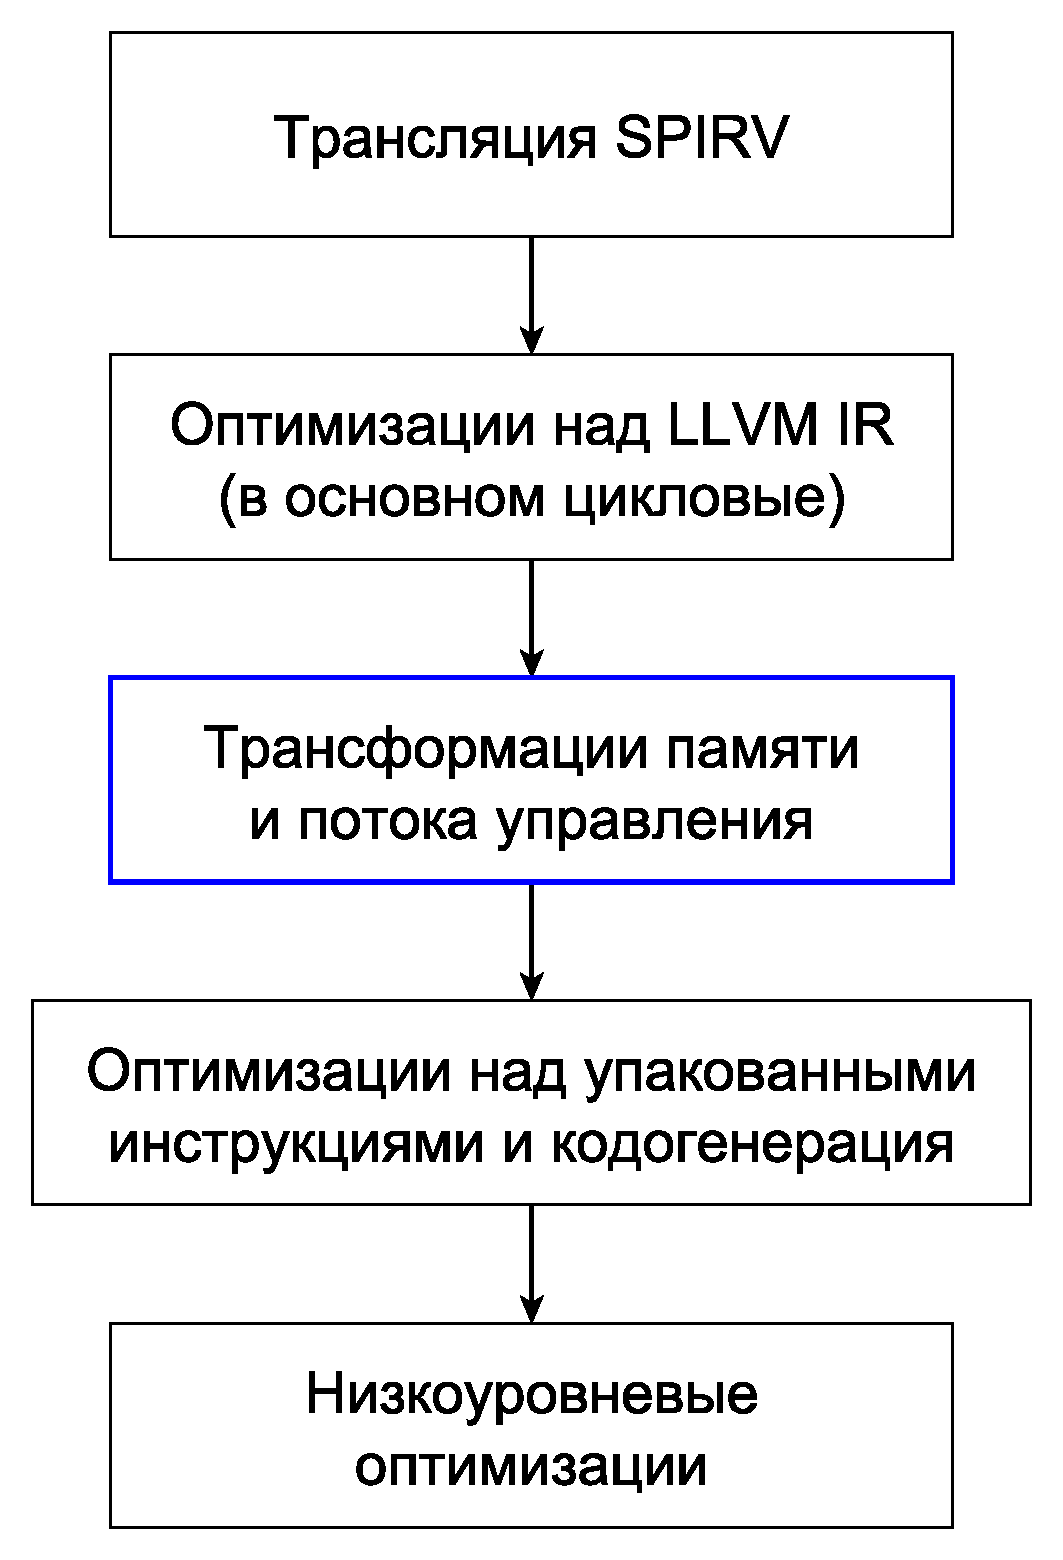
\includegraphics[scale=0.4]{Vladimirov/images/highlevel-mgr.pdf}
    }
    \caption{Высокоуровневый список трансформаций}\label{fig:highlevel-mgr}
\end{figure}

Высокоуровневая схема менеджера пассов представлена на рисунке~\cref{fig:highlevel-mgr}. Выбор места обосновывается как результатами экспериментов, так и следующими соображениями.

\begin{itemize}
\item Трансформация операций копирования возможна только после того как эта операция распознана как идиома, то есть после оптимизаций над высокоуровневым IR.
\item Разрешение адресных пространств может породить много платформенно-зависимого кода и должно идти до оптимизаций над легализованными инструкциями.
\item Трансформация приватных операций с памятью и выделение спиллов должно идти после цикловых оптимизаций, но до вставки пролога и эпилога.
\item TODO: расписать все соображения.
\end{itemize}

Важно подчеркнуть, что метод применим к любой системе и любому уровню промежуточного представления с минимальными модификациями. 

\begin{figure}[ht]
    \centerfloat{
        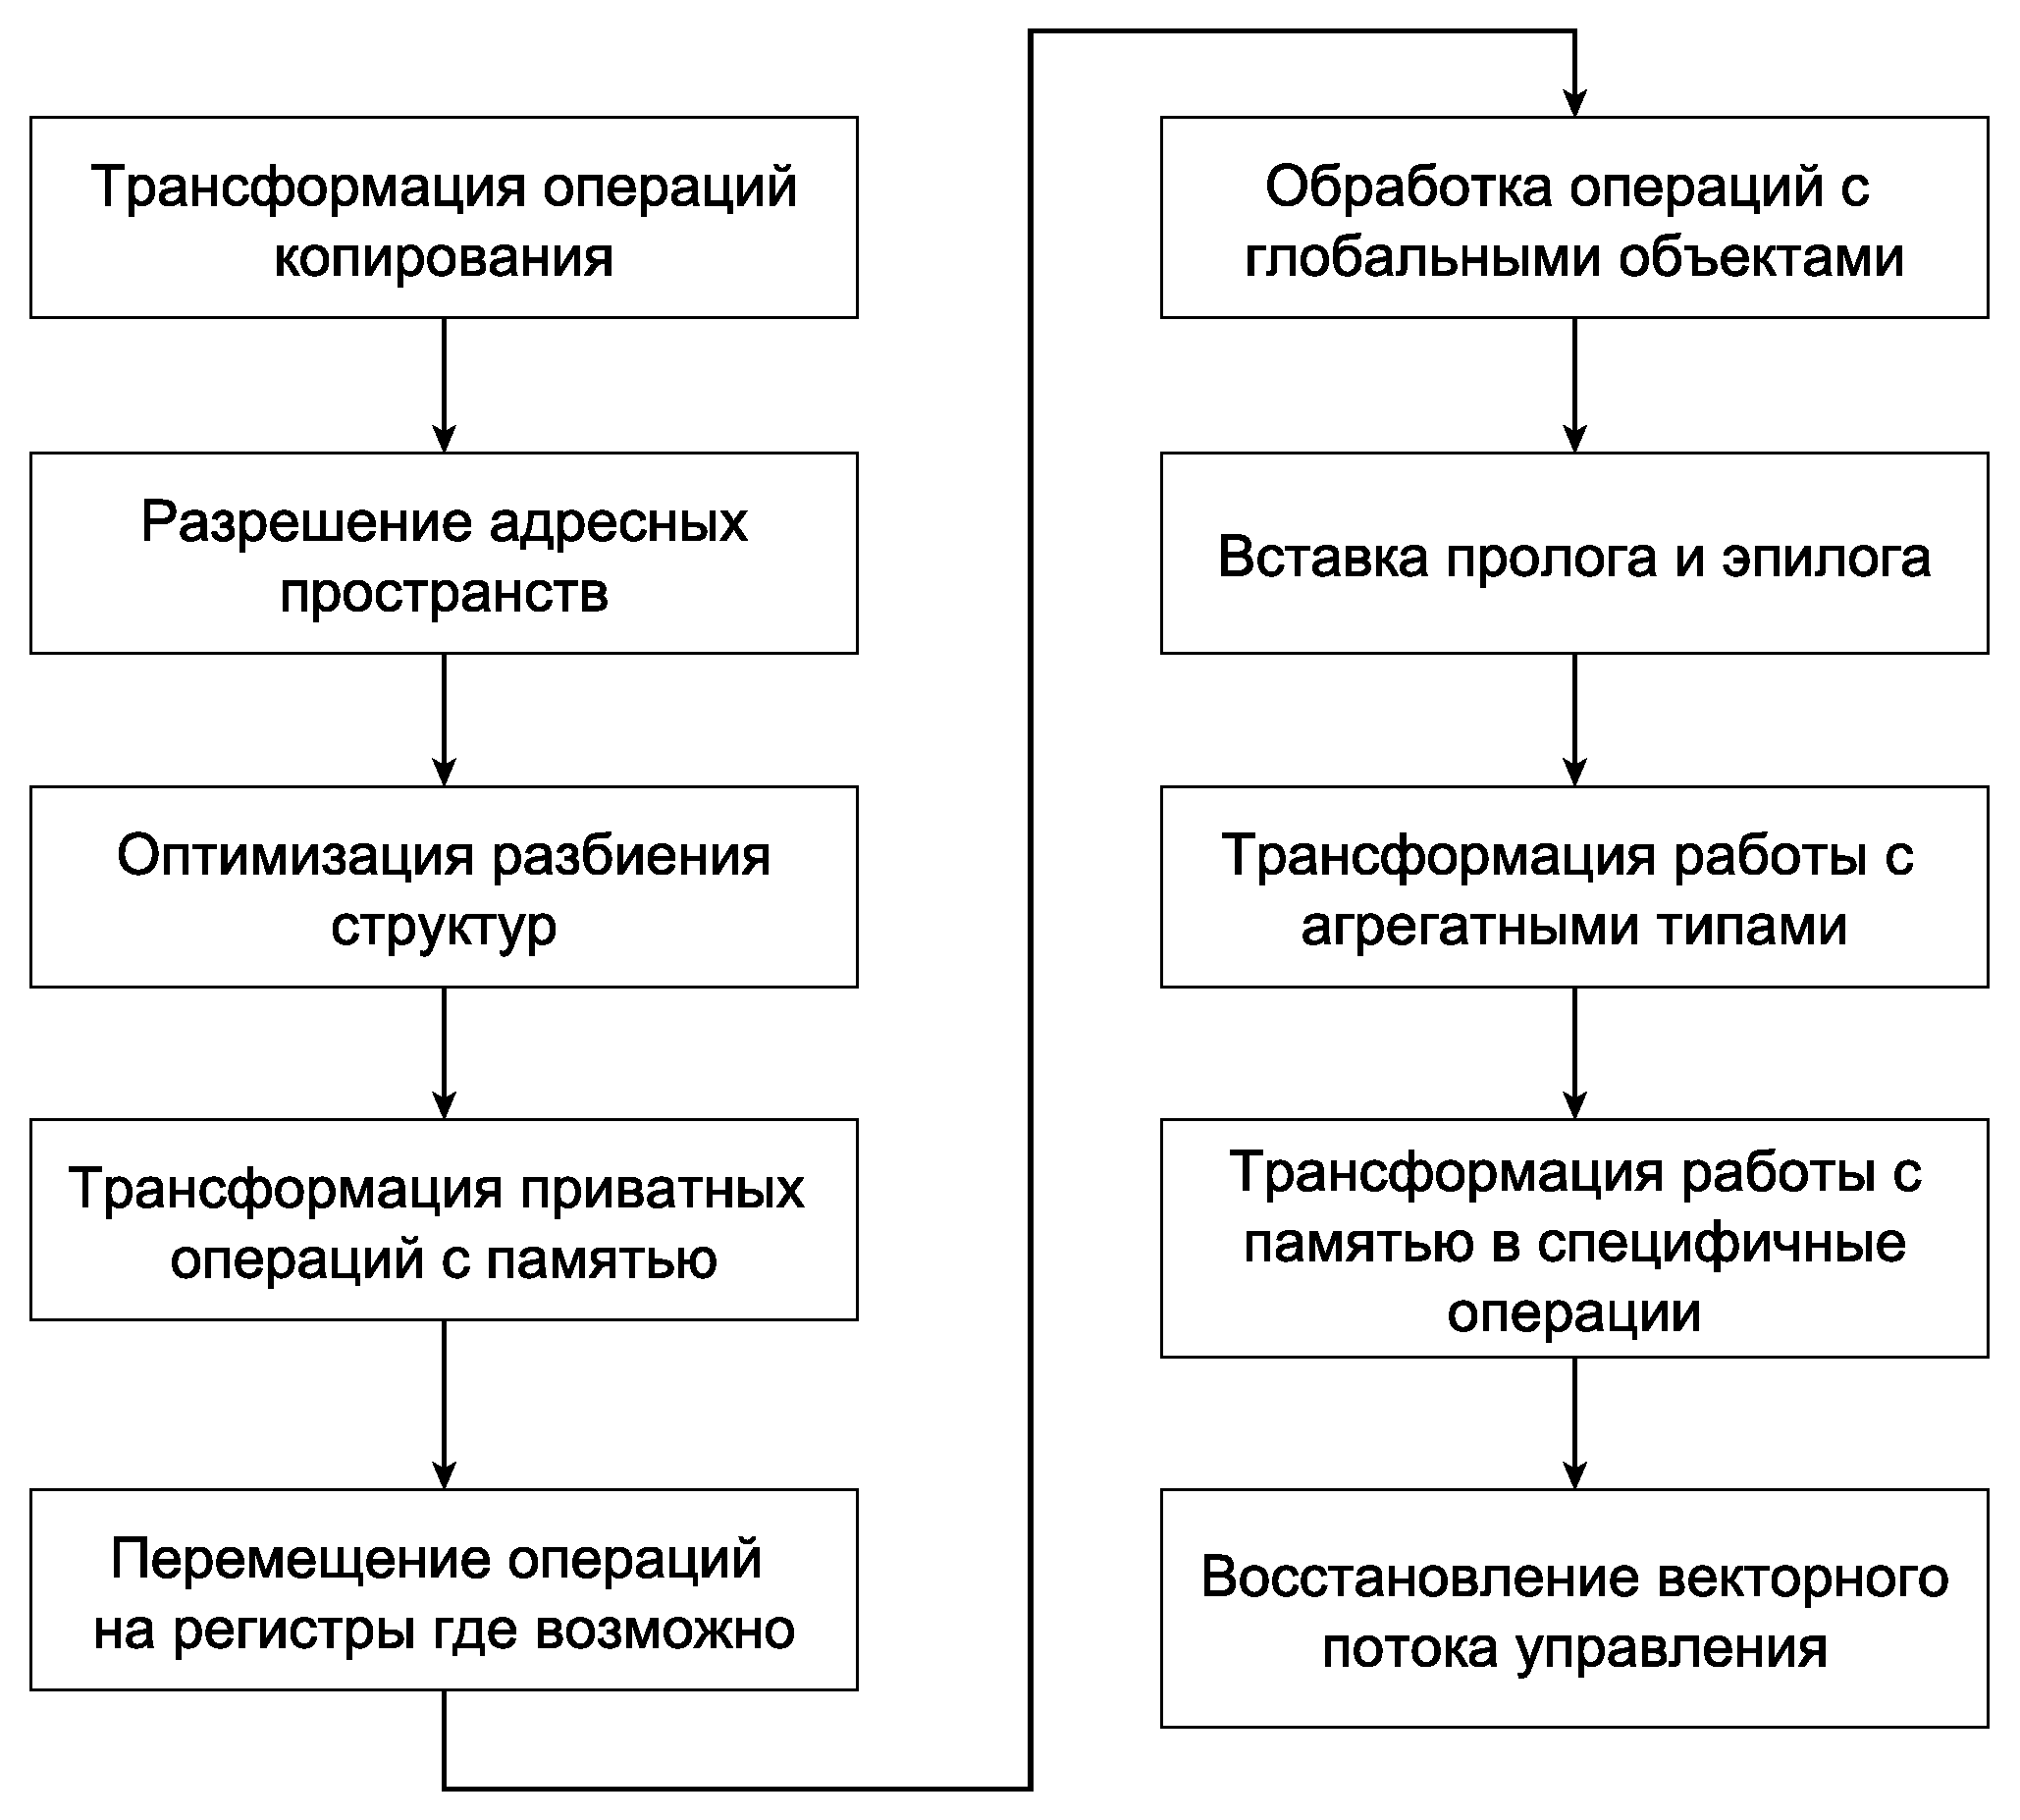
\includegraphics[scale=0.4]{Vladimirov/images/passmgr.pdf}
    }
    \caption{Детальный список трансформаций}\label{fig:passmgr}
\end{figure}

Детальный список трансформаций представлен на рисунке~\cref{fig:passmgr}. В нём есть два вида трансформаций -- обязательные легализации необходимые для представления высокоуровневых конструкций для векторной системы команд и необязательные оптимизации, которые оптимизируют представление, делая его более подходящим для высокоэффективных вычислений.

\subsection{Высокоуровневое представление}\label{subsec:lowering/passes/highlevel}

Представление на IR высокого уровня (HIR, high-level IR) после высокоуровневого языка содержит адресные пространства и трансформации типов указателей между типами пространств адресов. Кроме того там используются обобщённые операции загрузки и сохранения.

\begin{ListingEnv}[!h]
    \captiondelim{ } 
    \caption{Пример представления на HIR}\label{lst:lowering/irrep}
    \begin{Verb}
%4 = tail call i32 @llvm.genx.group.id.x()
%5 = extractelement <3 x i32> %local.size, i32 0
%6 = mul i32 %4, %5
%7 = extractelement <3 x i32> %local.id, i32 0
%8 = add i32 %6, %7
    \end{Verb}
\end{ListingEnv}

Листинг~\cref{lst:lowering/irrep} показывет загрузку вектора группового идентификатора, умножение на локальный размер и прибавление локального идентификатора как высокоуровневые операции.

\subsection{Инварианты трансформаций}\label{subsec:lowering/passes/invariants}

Предлагаемые трансформации имеют инварианты применения, представленные на рисунке~\cref{fig:highlevel-mgr-inv}. Поскольку предлагаемая методология является достаточно общей, важно понимать в каких случаях они могут быть ослаблены или усилены.

\begin{figure}[ht]
    \centerfloat{
        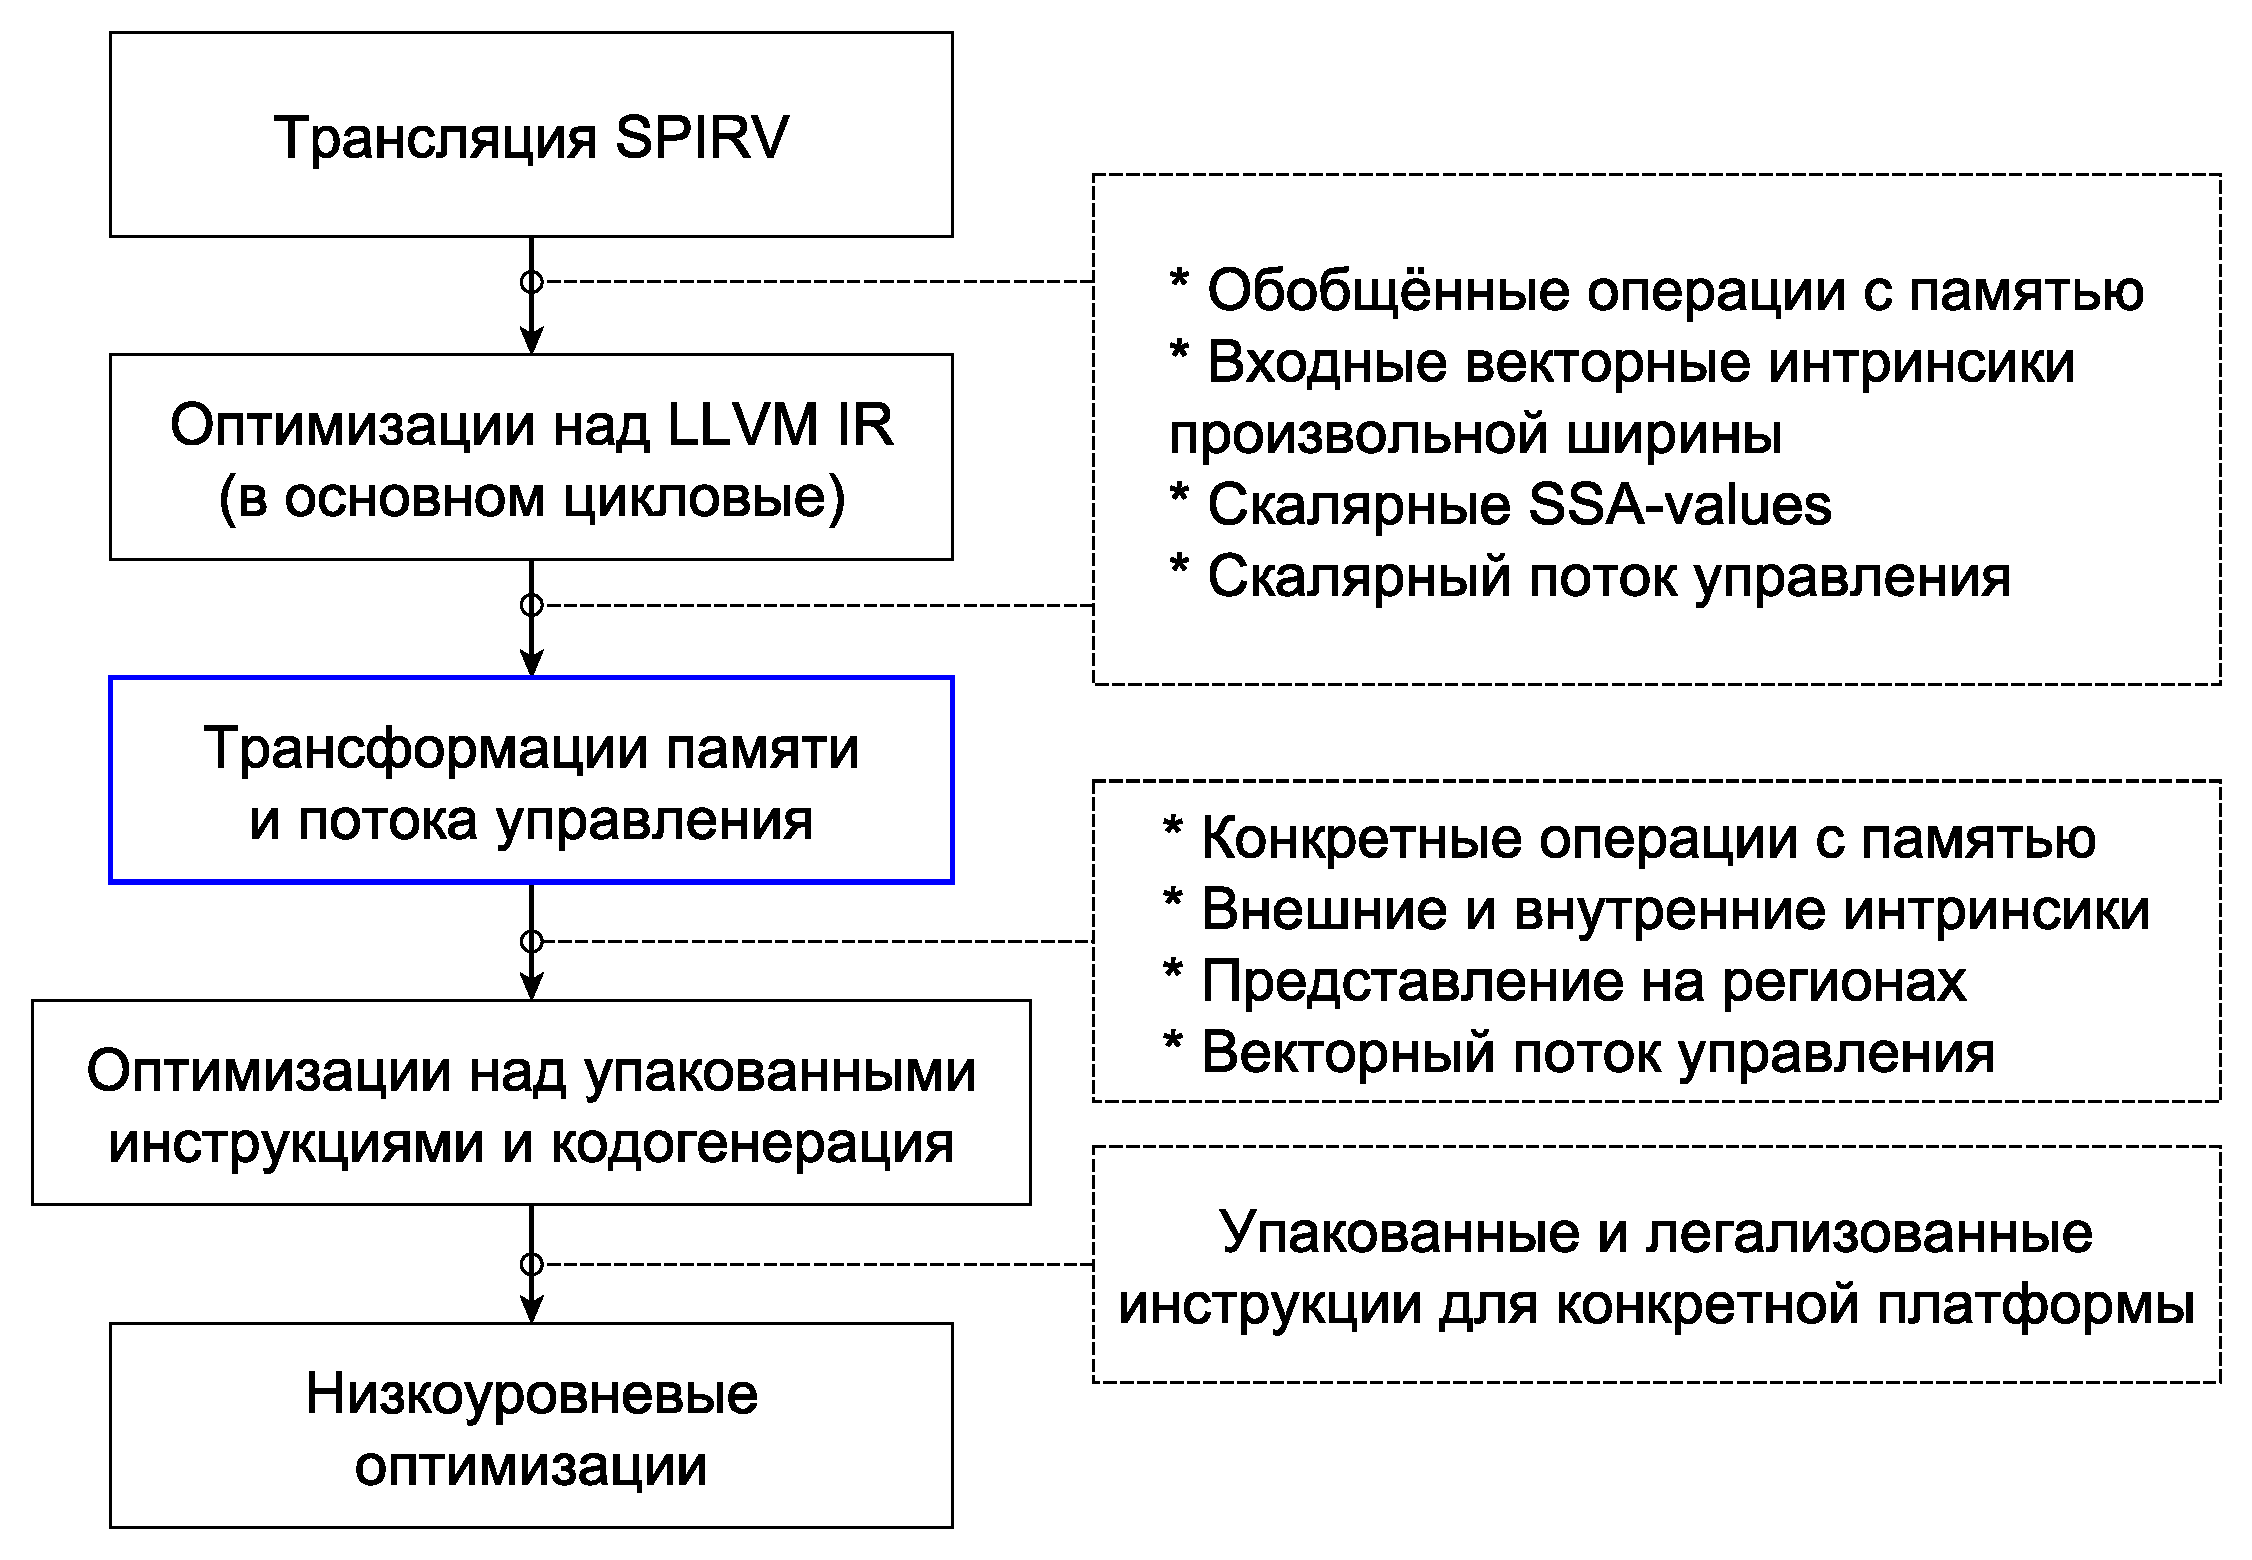
\includegraphics[scale=0.4]{Vladimirov/images/highlevel-mgr-inv.pdf}
    }
    \caption{Инварианты при трансформациях}\label{fig:highlevel-mgr-inv}
\end{figure}

После оптимизаций над высокоуровневым представлением, память не обязательно представляется исключительно обобщёнными операциями. Например программист может написать явный векторный код, работающий с векторными загрузками из памяти. В этом случае высокоуровневые оптимизации вряд ли будут способны обработать такую операцию и на вход каскадного понижения она попадёт в неизменном виде.

\subsection{Представление на регионах}\label{subsec:lowering/passes/lowlevel}

Физическое представление на регионах может существовать во многих формах. Например в графическом компиляторе Intel оно существует в виде G4IR, в виде VISA и в виде XeISA. 

\begin{ListingEnv}[!h]
    \captiondelim{ } 
    \caption{Пример физического представления}\label{lst:lowering/regrep}
    \begin{Verb}
mov (1|M0) r5.0<1>:uq r2.2<0;1,0>:uq
send (8|M0) r1 r5 0xC 0x021D0AFF
mov (1|M0) r6.0<1>:uq r2.3<0;1,0>:uq
send (8|M0) r3 r6 0xC 0x021D0AFF
add (8|M0) r4.0<1>:f r1.0<8;8,1>:f r3.0<8;8,1>:f
mov (1|M0) r7.0<1>:uq r2.1<0;1,0>:uq
sends (8|M0) r7 r4 0x4C 0x020D42FF
    \end{Verb}
\end{ListingEnv}

Листинг~\cref{lst:lowering/regrep} показывает типичное представление на регионах того же самого кода, который высокоуровнево представлен на листинге~\cref{lst:lowering/irrep}.

\section{Разбиение структур}\label{sec:lowering/splitter}

\subsection{Выделение частей агрегатных типов для векторизации}\label{subsec:lowering/splitter/vectorization}

Перед описанием алгоритма разбиения определим правила, по которым мы будем выделять части агрегатных типов для векторизации.

В стандарте C++ существует концепция скалярного типа. Скалярными называются арифметические типы, типы перечислений, указатели и cv-квалифицрованные версии перечисленных типов. Назовём \emph{базовым} скалярный тип, поддерживаемый данной оптимизацией. В это множество входят также векторные типы, которых нет в C++, но которые есть в LLVM IR.  В это множество не входят, например, указатели. Определение сознательно является несколько нечетким, чтобы заложить возможность будущего расширения. Алгоритм ниже не разбивает базовые типы.

Назовём \emph{примитивным} либо базовый тип, либо агрегатный тип, у которого типы всех элементов одинаковы и примитивны. Такой тип нет необходимости делить, так как объекты таких типов могут быть легко переделаны в вектора фазой aggregate lowering, которая представлена в векторном оптимизаторе IGC. Для алгоритма нет разницы между примитивным типом и базовым, из которого этот примитивный тип состоит, поэтому примитивный всегда будет сводиться к базовому. Например, \verb|< 3 x [ 5 x int]>| будет эквивалентен типу \verb|int|.

Целью алгоритма разбиения структур является приведение всех структур в модуле (например в модуле LLVM IR) к структурам примитивного типа с обязательным сохранением поведения исходной программы в рамках as-if rule.

Фаза разбиения структур в векторном компиляторе разрабатывалась специально для ISPC -- компилятора для SPMD~(single program, multiple data). При этом алгоритм сам по себе может быть использован в более широких классах оптимизаторов, даже не основанных на LLVM. Оптимизация работает над LLVM модулем и должна применятся до векторизации.

Разбиение невозможно, если:
\begin{enumerate}
\item элемент структуры является указателем на другую нетривиальную структуру, в том числе на саму себя.
\item на структуру взят указатель.
\end{enumerate}

Первое ограничение появляется из-за использования версии LLVM, в которой ещё не были введены opaque указатели.
Собственноручная поддержка таких указателей приводит к сильному разрастанию получаемого модуля и невозможности применения других оптимизаций.
По этой же причине была невозможна поддержка передачи структур в пользовательские функции.
Второе ограничение связано с тем, что замена кода работы с указателем на аналогичный код с поделёнными структурами может привести к значительному увеличению количества инструкций.

\subsection{Описание алгоритма}\label{subsec:lowering/splitter/algorithm}

\textbf{Шаг 1. Сбор информации о структурах в модуле}

Информация о структуре хранится в виде хэш-таблицы, где ключ -- это примитивный тип элемента, а значения -- элементы, соответствующие этому типу. Структура в дальнейшем будет делиться как раз по элементам этой хэш-таблицы, так как ключам будет соответствовать примитивный тип, а значениям -- элементы будущей структуры. 
Количество ключей минус один -- столько структур необходимо будет сгенерировать.
Соответственно, если у структуры существует только один примитивный тип, то данную структуру делить нет необходимости, так как она сама является примитивной.

\textbf{Шаг 2. Построение графа вложенности структур}

Так как элементами структуры могут быть другие структуры, то такие ситуации необходимо разрешать.
Граф строится следующим образом: вершине $A$ соответствует структура \%A.
Ребро от вершины $C$ в вершину $A$ проводится в том случае, если структура, соответствующая вершине $A$, вложена в структуру, соответствующую вершине $C$.
Назовём головой графа($Head$) вершины, которые соответствуют структурам, не вложенным ни в какие другие структуры.
Голов графа может быть как одна, так и несколько.

\textbf{Шаг 3. Обработка графа вложенности структур}

Обработка графа начинается с головы, однако деление -- с самой нижней вершины.
Все нижние вершины всегда характеризуются тем, что структуры, связанные с ними содержат элементы только примитивных типов, а значит данные структуры могут быть поделены.
При обработке вершины графа возможны два варианта.
Первое -- если вершина отвечает за примитивную структуру, то в делении нет необходимости и данная вершина удаляется из графа.
Второе -- структура, отвечающая за вершину была поделена.
Тогда нужно заменить во всех структурах, в которые была вложена данная, все элементы, отвечающие за данную структуру, на новые элементы с поделёнными структурами.
Во время замены элементов появляются промежуточные представления структур, которые затем необходимо удалить.
После обработки вершины она удаляется, поэтому все структуры будут обработаны тогда, когда весь граф удалится.

\textbf{Шаг 4. Обработка и замена инструкций}

Обработка инструкций всегда начинается с инструкции выделения памяти на стековом фрейме под структуру (AI -- alloca в LLVM IR).
Далее единственными допустимыми пользователями инструкций выделения памяти являются только инструкции обращения к элементу агрегата (GEP -- getelementptr).
Однако в нашей реализации были допущены инструкции приведения (bitcast) и ptrtoint (PTI) только с определёнными шаблонами использования.
В случае bitcast единственными пользователями могут быть только интринсики lifetime.start/end.
% TODO убрать зависимость от ISPC FE в описании алгоритма
В случае ptrtoint фронтенд ISPC вместо доступа к нулевому элементу структуры через getelementptr использует указатель на структуру.
Данный подход необходимо было поддерживать, поэтому в анализе ptrtoint проверяется соответствие шаблону вычисления указателя из следующих инструкций: insertelement, shufflevector, add и read/write.
В случае если результатом обращения к элементу является примитивный тип, то эта инструкция заменяется на эквивалентную с другим операндом и новой цепочкой индексов.
Если результатом является уже разбитая структура, то будут сгенерированы столько новых обращений, на сколько структур была разбита исходная.

\section{Восстановление векторного потока управления}\label{sec:lowering/simdcf}

\subsection{Интерфейс между языками высокого уровня и векторным компилятором}\label{sec:lowering/simdcf/intface}

Одним из языков, используемых для разработки программ исполняемых на видеокартах, является ISPC. ISPC (Implicit SPMD Program Compiler) - язык программирования, являющийся расширением С и реализующий концепцию SPMD (single program, multiple data). ISPC является языком с раздельным исходным кодом. Изначально целевой архитектурой для данного языка была только архитектура x86 с векторными расширениями, но позже была добавлена поддержка для ARM процессоров с расширениями Neon, а также графических ускорителей Intel XE.

Программа на языке ISPC является SPMD программой и компилируется для векторов заранее известной зафиксированной длины. В такой программе могут обрабатываться как общие для всех потоков данные, так и свои данные для каждого запущенного потока. Общие данные отмечают как uniform переменные (то есть не изменяющиеся в зависимости от векторной линии), остальные по умолчанию считаются varying (то есть изменяющиеся). Таким образом любую varying переменную можно рассматривать как элемент вектора.

На листинге 2 приведен пример функции на языке ISPC.

\begin{verbatim}
void simple(uniform float vin[],
            uniform float vout[],
            uniform int count) {
  foreach (index = 0 ... count) {
    float v = vin[index];
    if (v < 3.)
        v = v * v;
    else
        v = sqrt(v);
    vout[index] = v;
  }
}
\end{verbatim}

В ISPC нет ограничений на векторный поток управления. В стандартных конструкциях языка он реализуется через использование в качестве условия varying переменной. При этом, так как ISPC является кроссплатформенным (и поддерживаемые им архитектуры различаются действительно кардинально) использование платформенно-специфичных интринсиков нежелательно. Вместо этого ISPC маскирует результаты операций после условных переходов для векторного потока управления. Для архитектуры графических ускорителей Intel такой подход не позволяет использовать всех векторных возможностей потока управления, аппаратуры.

В связи с этим нами предлагается интефейс для языков высокого использующих векторный backend графического компилятора Intel. Так как интерфейс должен представлять собой конструкцию на промежуточном представлении LLVM IR, который не поддерживает векторный поток управления, неизбежно возникает необходимость сводить векторное условие к скалярному виду. Перед условным переходом необходимо проверить справедливо ли условие хоть для одного элемента и выполнять переход только в таком случае. Для наибольшей кроссплатформенности для подобных проверок следует использовать стандартные интринсики LLVM \texttt{@llvm.vector.reduce.and} и \texttt{@llvm.vector.reduce.or}. Также для языков высокого уровня, поддерживающих только архитектуру графических ускорителей Intel как целевую (например CM), допускается использовать для редукции условий платформозависимые интринсики \text{@llvm.genx.any} и \text{@llvm.genx.any}, являющиеся полными аналогами прежде упомянутых. Для сохранения семантического смысла и поддержки платформ, на которых нет развитой поддержки векторного потока управления, необходимо маскировать условием побочные эффекты дуги перехода.

Данный подход также применим для скалярных архитектур, поддерживающих необходимые минимальные векторные расширения. При этом в процессе оптимизаций компилятор не сможет сделать трансформации ломающие порядок побочных эффектов, поэтому такая конструкция будет валидна на всех этапах своего существования.

\subsection{Поиск конструкций векторного потока управления}\label{sec:lowering/simdcf/optimization}

После определения SIMD CF региона можно свести задачу поиска заранее оговоренных конструкций к поиску SIMD CF регионов самого внешнего уровня вложенности, после чего искать вложенные SIMD CF регионы.

Шаг 1. Поиск условного перехода, похожего на векторный поток управления. Для каждого базового блока проверяется его терминатор. Если это инструкция условного перехода, то проверяется его условие, в противном случае конструкция не является SIMD CF регионом. Если условием является результат вызова одного из обозначенных ранее интринсиков, то идет переход к шагу 2.

Шаг 2. Проверяется структура потока управления и происходит попытка сопоставить его либо с SIMD CF if/else, либо с SIMD CF циклом. Если сопоставление с одним из заданных паттернов невозможно, то конструкция не является SIMD CF регионом. В противном случае происходит переход к шагу 3.

Шаг 3. Проверка маскирования побочных эффектов. Для каждой инструкции, у которой есть побочные эффекты проводится проверка, является ли такая инструкция маскирована и если она маскирована, то проверяется, совпадает ли маска для данной инструкции с условием перехода в эту дугу. Для вложенных регионов проверяется, является ли маска данного региона подмножеством маски внешнего региона. Если проверка неудачная - данный регион не является SIMD CF регионом.

Дополнение к шагу 3 для цикла. Проверяются фи-узлы для индуктивностей и пересчет маски для каждого цикла. Если проверка неудачная - данный регион не является SIMD CF регионом. В противном случае идет переход к шагу 4.

Дополнение к шагу 3 для if-else. Если кроме if также имеется else, то происходит проверка, являются ли маски if и else строго противоположны друг другу. Если проверка неудачная - данный регион не является SIMD CF регионом. В противном случае идет переход к шагу 4.

Шаг 4. Данный регион является SIMD CF регионом. Аналогично происходит поиск вложенных SIMD CF регионов для данного региона.

В псевдокоде данный алгоритм будет выглядеть как показано на листинге~\ref{lst:simdcf-analysis}

\subsection{Трансформация конструкций векторного потока управления}\label{sec:lowering/simdcf/optimization}

После сбора всей информации о SIMD CF регионах начинается их оптимизирующая трансформация.

TODO: картинки и трансформация

\section{Выводы}\label{sec:lowering/outcome}

Во второй главе описывается метод ступенчатого понижения промежуточного представления, алгоритм разбиения структур и алгоритм восстановления векторного потока управления.

При описании метода ступенчатого понижения, описываются его основные ограничения и допущения. Метод состоит из нескольких трансформаций, трансформации разбиты на функциональные и оптимизационные. Каждая трансформация подробно рассматривается, указывается её место в общей картине и взаимодействие с другими трансформациями. Описываются инварианты трансформаций, а также их входной и выходной формат: обобщённое высокоуровневое представление и представление на регионах.

При описании алгоритма восстановления векторного потока управления описывается интерфейс между языками высокого уровня и векторным компилятором, мотивируется почему этот интерфейс должен быть скалярным и предикатным. Далее описывается в общих чертах алгоритм восстановления векторного потока управления (детально он описан в прложении). После того как основные конструкции распознаны, описывается трансформация, восстанавливающая их в оптимизаторе.

При описании алгоритма разбиения структур описывается механизм выделения частей агрегатных типов для векторизации. Далее в деталях описывается сам алгоритм разбиения структур, включающий построение графа вложенности и нетривиальную обработку этого графа.

\FloatBarrier           % Глава 2
\chapter{Реализация и результаты экспериментов}\label{ch:results}

\section{Инфраструктура компилятора LLVM}\label{sec:results/llvm}

Тут про то что LLVM это индустриальный стандарт \cite{lattner2005llvm}.

Компиляторная инфраструктура LLVM часто используется в HPC проектах, см. \cite{tian2016llvm} и \cite{tian2017llvm}.

LLVM поддерживает много уровней машинного представления \cite{racordon2021asts}.

В конмпиляторной инфраструктуре LLVM заложена достаточная гибкость, чтобы использовать как высокоуровневые оптимизации над промежуточным представлением, так и низкоуровневые, специфичные для конкретных языков программирования \cite{lee2018reconciling}.

\subsection{Особенности LLVM IR}\label{subsec:results/llvm/ir}

Одним из сильных преимуществ LLVM является промежуточное машинно-независимое представление кода (\textit{Intermediate Representation -- IR}), которое использует миддлэнд для оптимизаций (и которое является выходным форматом для фронтенда и входным для бэкенда). Промежуточное представление LLVM может использоваться в трёх разных формах: как набор структур данных для представления кода в памяти во время компиляции, сериализовываться в виде бинарного кода для хранения на диске (\textit{LLVM bitcode}), и в текстовом виде для удобного чтения и анализа. Все эти формы LLVM IR являются эквивалентными. На самом высоком уровне LLVM оперирует с модулями, что к примеру соответствует концепции единицы трансляции (\textit{translation unit}) языков C и C++. Каждый модуль состоит из глобальных переменных и функций (идентификаторы глобальных объектов всегда начинаются с символа '@'), а также из таблицы метаданных. Объявление функции начинается со слова declare и содержит возвращаемый тип, имя функции, список аргументов и может содержать некоторые опциональные атрибуты; определение функции начинается со слова define и помимо прочего ещё содержит список базовых блоков, которые образуют CFG. Первый блок всегда является точкой входа и не может иметь предшественников (и поэтому также не может иметь $\varphi$-функции). В свою очередь каждый базовый блок начинается с опциональной метки (если она не указана явно, метка с номером назначается автоматически) и списка инструкций, которые заканчиваются инструкцией-терминатором (такой как инструкция перехода или возврат из функции). LLVM IR использует SSA-представление, и это означает, что инструкция может отождествляться со значением которое оно определяет (так как оно единственное). Идентификаторы локальных объектов (такие как значения инструкций) начинаются с символа '\%'. $\varphi$-функции представляются в виде отдельных инструкций (PHINode), которые должны следовать в начале базового блока перед всеми остальными инструкциями.

\begin{ListingEnv}[!h]
    \captiondelim{ } 
    \caption{Пример LLVM IR}\label{lst:results/llvmir}
    \begin{lstlisting}[language=llvm]
; Example of factorial:
; int factorial(int n) {
;  return n ? n * factorial(n - 1) : 1;
; }

define i32 @factorial(i32) {
entry:
  %ne = icmp ne i32 %0, 0
  br i1 %ne, label %then, label %exit

then:   ; preds = %entry
  %sub = sub i32 %0, 1
  %2 = call i32 @factorial(i32 %sub)
  %mult = mul i32 %0, %2
  br label %exit

exit: ; preds = %entry, %then
  %res = phi i32 [ 1, %entry ], [ %mult, %then ]
  ret i32 %res
}
    \end{lstlisting}
\end{ListingEnv}

На листинге~\cref{lst:results/llvmir} приведен пример LLVM IR. Это промежуточное представление является строго типизированным, что позволяет осуществлять напрямую некоторые типы оптимизаций. В качестве базовых типов присутствуют целочисленный тип ($i_N$, где $N$ -- количество бит, например $i_32$), типы чисел с плавающей запятой (half, float, double, а также некоторые платформо-специфичные, например x86\_fp80), указатели вида \lstinline!<type> *! (указатели на конкретный тип) и недавно добавленные в LLVM <<прозрачные>> (opaque) указатели без типа (обозначаются ptr), а также векторные типы (синтаксис \lstinline!<NumElems x ElemType>!, например \lstinline!<8 x i32>!). Агрегатными типами являются массивы (синтаксис \lstinline![NumElems x ElemType]!, например \lstinline![40 x i8]!) и структуры (синтаксис \lstinline!type { <type list> }!, например \lstinline!{float, i8, i32}!).

\subsection{Платформенно независимые оптимизации}\label{subsec:results/llvm/opts}

Тут про то как хорошо LLVM оптимизирует циклы.
\cite{sarkar2000optimized}

Существенной проблемой является неопределенное поведение, проникающее из языков высокого уровня. К счастью в LLVM IR есть эффективные средства работы с таким поведением \cite{lee2017taming}.

\section{Реализация в IGC}\label{sec:results/igc}

Тут про IGC в целом

\subsection{Особенности промежуточного представления в IGC}\label{subsec:results/igc/ir}

Для эффективного распределения регистров, IGC использует ещё более низкоуровневое представление -- G4IR \cite{chen2018register}.

\subsection{Детали обработки разбиения структур в IGC}\label{subsec:results/igc/splitted}

Обработка инструкций всегда начинается с инструкции выделения памяти на стековом фрейме под структуру (AI -- alloca в LLVM IR).
Далее единственными допустимыми пользователями инструкций выделения памяти являются только инструкции обращения к элементу агрегата (GEP -- getelementptr).
Однако в нашей реализации были допущены инструкции приведения (bitcast) и ptrtoint (PTI) только с определёнными шаблонами использования.
В случае bitcast единственными пользователями могут быть только интринсики lifetime.start/end.
% TODO убрать зависимость от ISPC FE в описании алгоритма
В случае ptrtoint фронтенд ISPC вместо доступа к нулевому элементу структуры через getelementptr использует указатель на структуру.
Данный подход необходимо было поддерживать, поэтому в анализе ptrtoint проверяется соответствие шаблону вычисления указателя из следующих инструкций: insertelement, shufflevector, add и read/write.
В случае если результатом обращения к элементу является примитивный тип, то эта инструкция заменяется на эквивалентную с другим операндом и новой цепочкой индексов.
Если результатом является уже разбитая структура, то будут сгенерированы столько новых обращений, на сколько структур была разбита исходная.


\section{Методология замеров}\label{sec:results/measures}

Тут про замеры графических шейдеров

\section{Результаты замеров}\label{sec:results/results}

\subsection{Результаты ступенчатого понижения}\label{subsec:results/results/lowering}

Результаты сведены в таблицу~\cref{tab:results/lowering}. В ней введены следующие сокращения.

\begin{itemize}
\item \textbf{P} Пакет тестов в ESIMD тестировании
\item \textbf{T} Трансформации приватных операций
\item \textbf{G} Операции с глобальными объектами
\item \textbf{A} Трансформация агрегатных типов
\item \textbf{M} Понижение уровня операций работы с памятью
\item \textbf{Pass} Пакет начал проходить с новым конвеером
\end{itemize}

\begin{table}[!h]
    \centering
    \captionsetup{justification=centering}
    \caption{Результаты ступенчатого понижения}\label{tab:results/lowering}
    \begin{tabular}{|p{0.24\linewidth}|p{0.1\linewidth}|p{0.1\linewidth}|p{0.1\linewidth}|p{0.1\linewidth}|p{0.1\linewidth}|}
        \hline
        P & T & G & A & M & Pass \\ \hline        
        glob   & \verb|+| & \verb|+| & \verb|-| & \verb|-| & \verb|+| \\ \hline
        dpas   & \verb|+| & \verb|-| & \verb|+| & \verb|+| & \verb|+| \\ \hline
        lsc    & \verb|+| & \verb|-| & \verb|+| & \verb|-| & \verb|~| \\ \hline
        atomic & \verb|-| & \verb|+| & \verb|-| & \verb|+| & \verb|~| \\ \hline
        slm    & \verb|-| & \verb|-| & \verb|-| & \verb|+| & \verb|+| \\ \hline
        vec\_arg\_call\_conv & 
                 \verb|+| & \verb|+| & \verb|-| & \verb|-| & \verb|+| \\ \hline
        gather\_scatter    & 
                 \verb|-| & \verb|-| & \verb|+| & \verb|+| & \verb|+| \\ \hline
        ctor\_codegen      & 
                 \verb|-| & \verb|-| & \verb|-| & \verb|+| & \verb|+| \\ \hline
        simd\_copy & 
                 \verb|+| & \verb|+| & \verb|-| & \verb|+| & \verb|~| \\ \hline
    \end{tabular}
\end{table}

\subsection{Результаты разбиения структур}\label{subsec:results/results/splitter}

Для тестирования алгоритма разбиения структур использовались приложения из открытого стека рендеринга Intel (OSPray, Embree). Была оценена корректность алгоритма (прошли все тесты) и его положительное влияние на производительность скомпилированной программы.

Результаты сведены в таблицу~\cref{tab:results/splitter}.

\begin{table}
    \centering
    \captionsetup{justification=centering}
    \caption{Результаты разбиения структур}\label{tab:results/splitter}
    \begin{tabular}{llc|llc}
        \toprule
        Бенчмарк & Результат & Результат \\
        \midrule
        Первый   & \verb|+|  & \verb|+|  \\
        Второй   & \verb| |  & \verb|+|  \\
        Третий   & \verb|+|  & \verb| |  \\
        \bottomrule
    \end{tabular}
\end{table}

\subsection{Результаты восстановления векторного потока управления}\label{subsec:results/results/simdcf}

Результаты сведены в таблицу~\cref{tab:results/simdcf}.

\begin{table}
    \centering
    \captionsetup{justification=centering}
    \caption{Результаты восстановления векторного потока управления}\label{tab:results/simdcf}
    \begin{tabular}{llc|llc}
        \toprule
        Бенчмарк & Результат & Результат \\
        \midrule
        Первый   & \verb|+|  & \verb|+|  \\
        Второй   & \verb| |  & \verb|+|  \\
        Третий   & \verb|+|  & \verb| |  \\
        \bottomrule
    \end{tabular}
\end{table}

\section{Выводы}\label{sec:results/outcome}

В третьей главе описываются детали реализации и результаты экспеиментов.

Сначала описывается компиляторная инфраструктура LLVM в которой далее проводятся все эксперименты. Далее описываются особенности графического компилятора IGC и его место в графическом стеке. Отдельно рассматриваются вопросы замеров результатов исполнения шейдерного кода и описывается методология их получения и аппаратная поддержка для этого в современных архитектурах.

Далее описываются основные результаты экспериментов. Результаты применения метода ступенчатого понижения состоят в функциональной корректности работы пакетов тестов. Результаты алгоритмов разбиения структур и восстановления векторного потока управления это улучшение производительности приложений.

\FloatBarrier           % Глава 3
\chapter*{Заключение}                       % Заголовок
\addcontentsline{toc}{chapter}{Заключение}  % Добавляем его в оглавление

%% Согласно ГОСТ Р 7.0.11-2011:
%% 5.3.3 В заключении диссертации излагают итоги выполненного исследования, рекомендации, перспективы дальнейшей разработки темы.
%% 9.2.3 В заключении автореферата диссертации излагают итоги данного исследования, рекомендации и перспективы дальнейшей разработки темы.
%% Поэтому имеет смысл сделать эту часть общей и загрузить из одного файла в автореферат и в диссертацию:

Основные результаты работы заключаются в следующем.

\begin{enumerate}[beginpenalty=10000] % https://tex.stackexchange.com/a/476052/104425
  \item Разработана методология представления высокоуровневых векторных конструкций в векторной системе команд. Указанная методология применена к компилятору IGC.
  \item Разработан алгоритм разбиения структур данных для улучшения векторизации.
  \item Разработан алгоритм восстановления векторного потока управления.
  \item Получены результаты как по корректности так и по производительности кода.
\end{enumerate}

Таким образом, в диссертационной работе исследованы и разработаны методология и алгоритмы для повышения эффективности ключевых приложений в гетерогенных системах, что имеет существенное значение для области вычислений на графических ускорителях.

Перспективы дальнейшей разработки темы данной диссертации не ограничиваются графическими системами. В данный момент автор работает над масштабированием своих идей на кластеры RISCV процессоров в том числе с векторными расширениями.      % Заключение
\printnomenclature[3.5cm] % Значение ширины столбца с обозначениями стоит подбирать вручную
        % Список сокращений и условных обозначений

\iffalse
\include{Vladimirov/dictionary}      % Словарь терминов
\fi

\clearpage                                  % В том числе гарантирует, что список литературы в оглавлении будет с правильным номером страницы
%\hypersetup{ urlcolor=black }               % Ссылки делаем чёрными
%\providecommand*{\BibDash}{}                % В стилях ugost2008 отключаем использование тире как разделителя
\urlstyle{rm}                               % ссылки URL обычным шрифтом
\ifdefmacro{\microtypesetup}{\microtypesetup{protrusion=false}}{} % не рекомендуется применять пакет микротипографики к автоматически генерируемому списку литературы
\insertbibliofull                           % Подключаем Bib-базы: все статьи единым списком
% Режим с подсписками
%\insertbiblioexternal                      % Подключаем Bib-базы: статьи, не являющиеся статьями автора по теме диссертации
% Для вывода выберите и расскомментируйте одно из двух
%\insertbiblioauthor                        % Подключаем Bib-базы: работы автора единым списком 
%\insertbiblioauthorgrouped                 % Подключаем Bib-базы: работы автора сгруппированные (ВАК, WoS, Scopus и т.д.)
\ifdefmacro{\microtypesetup}{\microtypesetup{protrusion=true}}{}
\urlstyle{tt}                               % возвращаем установки шрифта ссылок URL
%\hypersetup{ urlcolor={urlcolor} }          % Восстанавливаем цвет ссылок
      % Список литературы
\clearpage
\ifdefmacro{\microtypesetup}{\microtypesetup{protrusion=false}}{} % не рекомендуется применять пакет микротипографики к автоматически генерируемым спискам
\listoffigures  % Список изображений

%%% Список таблиц %%%
% (ГОСТ Р 7.0.11-2011, 5.3.10)
\clearpage
\listoftables   % Список таблиц
\ifdefmacro{\microtypesetup}{\microtypesetup{protrusion=true}}{}
\newpage           % Списки таблиц и изображений (иллюстративный материал)

\setcounter{totalchapter}{\value{chapter}} % Подсчёт количества глав

%%% Настройки для приложений
\appendix
% Оформление заголовков приложений ближе к ГОСТ:
\setlength{\midchapskip}{20pt}
\renewcommand*{\afterchapternum}{\par\nobreak\vskip \midchapskip}
\renewcommand\thechapter{\Asbuk{chapter}} % Чтобы приложения русскими буквами нумеровались

\chapter{Алгоритм восстановления SIMD CF}\label{app:A}

\begin{ListingEnv}[!h]
    \captiondelim{ } 
    \caption{Анализ векторных управляющих конcтрукций, часть 1}\label{lst:simdcf-analysis}
    \begin{Verb}
procedure Find_SIMD_CF_Regions(Reg) returns set of SIMD_CF_Region
  Reg: Region
begin
  regions: set of SIMD_CF_Region
  bb: Basic_Block
  for each bb in Reg do
    if Is_SIMD_CF_Branch(bb.terminator) then
      match: SIMD_CF_Region
      match := Match(bb)
      if match then
        if Verify(match) then
          regions append match
        fi
      fi
    fi
  od
  return regions
end

procedure Is_SIMD_CF_Branch(Term) return boolean
  Term: Instruction
begin
  cond: Instruction
  cond := Term.condition
  return cond in {llvm.vector.reduce.and, llvm.vector.reduce.or}
end
    \end{Verb}
\end{ListingEnv}

\begin{ListingEnv}[!h]
    \captiondelim{ } 
    \caption{Анализ векторных управляющих конcтрукций, часть 2}
    \begin{Verb}
procedure Match(BB) return SIMD_CF_Region
  BB: Basic_Block
begin
  if MatchIf(BB) then
    return SIMD_CF_If_Region(BB)
  elif MatchLoop(BB) then
    return SIMD_CF_Loop_Region(BB)
  else
    return nil
end

procedure MatchIf(Entry) return SIMD_CF_If_Region
  Entry: Basic_Block
begin
  subregions: set of SIMD_CF_Region
  has_else: boolean
  if_begin, if_end, else_begin, else_end: Basic_Block
  exit: Basic_Block
  if_begin := Entry.true_succ
  else_begin := Entry.false_succ
  pred: Basic_Block
  for each pred in else_begin.preds do
    if pred != Entry then
      if_end := pred
    fi
  od
  subregions append Find_SIMD_CF_Regions(Region(if_begin, if_end))
  if !if_end.terminator.conditional then
    has_else := false
    exit := else_begin
    return SIMD_CF_If_Region(Entry, exit, has_else, subregions)
  fi
  has_else := true
  exit := if_end.false_succ
  for each pred in exit.preds do
    if pred != if_end then
      else_end := pred
    fi
  od
  subregions append Find_SIMD_CF_Regions(Region(else_begin, else_end))
  return SIMD_CF_If_Region(Entry, exit, has_else, subregions)
end
    \end{Verb}
\end{ListingEnv}

\begin{ListingEnv}[!h]
    \captiondelim{ } 
    \caption{Анализ векторных управляющих конcтрукций, часть 3}
    \begin{Verb}
procedure MatchLoop(BranchingBB) return SIMD_CF_Loop_Region
  BranchingBB: Basic_Block
begin
  loop: Loop
  loop := Get_Loop(BranchingBB)
  if !loop then
    return nil
  fi
  subregions append Find_SIMD_CF_Regions(Region(loop.entering, loop.exiting))
  return SIMD_CF_Loop_Region(loop, subregions)
end

procedure Verify(R) return boolean
  R: SIMD_CF_Region
begin
  inst: Instruction
  subreg: SIMD_CF_Region
  for each inst in R do
    if inst.has_side_effects and inst.mask != R.mask then
      return false     
    fi
  od
  for each subreg in R.subregions do
    if !R.is_submask(subreg_mask) then
      return false
    fi
  od
  return true
end
    \end{Verb}
\end{ListingEnv}
        % Приложения

\setcounter{totalappendix}{\value{chapter}} % Подсчёт количества приложений

\end{document}
